\chapter {Desenvolvimento}

Este capítulo tem como objetivo apresentar de forma detalhada a forma como se deu o desenvolvimento dos ajustes na funcionalidade de Texto Participativo. O desenvolvimento foi caracterizado pela sua forma incremental inspirado na metodologia ágil; na Seção \ref{sec:organizacao-do-desenvolvimento} é explicada as principais características da metodologia de trabalho. Uma série de requisitos que são discutidos na Seção \ref{sec:requisitos-iniciais} foram levantados para compor o ponto de partida do desenvolvimento. Uma breve contextualização do estado inicial da funcionalidade na plataforma é feito na Seção \ref{sec:contextualizacao-da-ferramenta-de-textos-participativos}. A Seção \ref{sec:etapas-de-desenvolvimento} traz uma visão cronológica das atividades realizadas, descrevendo a abordagem utilizada e a tomada de decisões realizada em cada momento. Na Seção \ref{sec:resultados} são apresentados os resultados obtidos, tanto de forma quantitativa quanto qualitativa.

\section {Organização do Desenvolvimento}
\label{sec:organizacao-do-desenvolvimento}

A organização do trabalho seguiu um modelo inspirado no desenvolvimento ágil, onde novas alterações eram feitas a cada \textit{sprint} e validada com o time de produto do Lab Livre e com os \textit{stakeholders} do projeto. Ao final de cada \textit{sprint}, após a validação do desenvolvimento realizado, com base nos \textit{feedbacks} do time de produto o desenvolvimento seguia para um novo objetivo: corrigir e alterar algo ou adicionar mais funcionalidades.

\section {Requisitos Iniciais}
\label{sec:requisitos-iniciais}

O desenvolvimento teve inicio com um conjunto de requisitos levantados pelos \textit{stakeholders} da Presidência que foram posteriormente trabalhados pelo time de produto do Lab Livre. No contexto político que se encontrava a plataforma Brasil Participativo, havia, principalmente, a necessidade de trazer aspectos de uma funcionalidade semelhante da plataforma Participa+ Brasil, que também é uma plataforma de participação social do governo federal. No Participa+ Brasil, o usuário administrador submetia o texto copiando e colando.

*

\section {Contextualização da Ferramenta de Textos Participativos}
\label{sec:contextualizacao-da-ferramenta-de-textos-participativos}

O texto participativo.

\section {Etapas de Desenvolvimento}
\label{sec:etapas-de-desenvolvimento}

No desenvolvimento dos ajustes e melhorias na ferramenta de textos participativos, no total houveram quatro \textit{sprints} de desenvolvimento, com duração média de um mês. Cada uma delas foi guiada pelos requisitos específicos levantados para aquele momento de trabalho, além dos \textit{feedbacks} fornecidos pelos usuários e pelo time de produto do Lab Livre.

\subsection {Sprint 1}

A \textit{Sprint} 1 pode ser caracterizada pelo início dos trabalhos, onde houve foco nos três requisitos que eram centrais na proposta de melhoria do componente:

\begin{itemize}
	\item \textbf{Requisito 1 da Sprint 1}: Diminuir o tempo de renderização da página de visualização do texto participativo;
	\item \textbf{Requisito 2 da Sprint 1}: Possibilitar a criação de textos participativos através de um editor de textos próprio do Brasil Participativo, contando com o uso do comando copiar e colar, trazendo texto de fontes como o Microsoft Word e Google Docs;
	\item \textbf{Requisito 3 da Sprint 1}: Refatoração da página de visualização do rascunho (edição de parágrafos), trazendo-a para o mesmo padrão de \textit{design} que a tela de visualização.
\end{itemize}

De acordo com o time de produto  do Lab Livre, o objetivo central era fazer um \textit{Minimum Viable Product} (MVP) para servir como uma espécie de prova de conceito, onde analisariam os resultados obtidos para eventualmente tomar uma decisão de manter ou não a mesma estratégia, a fim satisfazer as necessidades levantadas pelos \textit{stakeholders}. As próximas seções revelam detalhes da abordagem utilizada no desenvolvimento de cada requisito que foi listado acima.

\subsubsection {Requisito 1 da Sprint 1}

Aplicações \textit{Ruby on Rails} possuem um sistema de \textit{logs} que permitem que o desenvolvedor obtenha informações da execução de vários tipos e em vários níveis de detalhamento, sendo eles:

\begin{itemize}
	\item \textit{debug};
	\item \textit{info};
	\item \textit{warn};
	\item \textit{error};
	\item \textit{fatal};
	\item \textit{unknown}.
\end{itemize}

Por padrão, aplicações \textit{Rails} executadas em modo de desenvolvimento terão seu nível de \textit{log} como \textit{debug}, e quando executada em modo produtivo será \textit{info} \cite{debugging-rails-applications}.

Na condução dessa análise, o Brasil Participativo foi executado em modo desenvolvimento com nível de \textit{logs} como \textit{debug}. Com esse nível de informações, é possível visualizar na saída padrão do Puma quais consultas SQL estão sendo executadas, quais \textit{views} estão sendo renderizadas pelo \textit{Rails} durante a requisição e acessos ao ActiveStorage. Alguns desses registros são acompanhados pelo tempo gasto na execução e em alguns casos a quantidade de alocações também é informada.

Para realizar o primeiro diagnóstico, foi criado um texto participativo com em torno de 600 parágrafos, em seguida foi acessada a página de visualização do texto. A Figura \ref{fig:analise-log-600-paragrafos} mostra os \textit{logs} apresentados pela aplicação no processamento da requisição. Nota-se que a maior parte do tempo foi utilizado na renderização da \textit{views} e suas \textit{partials}, correspondendo a 96,7\% do tempo total gasto para processar a requisição.

\begin{figure}[htbp]
  \centering
  \caption{Captura de tela dos \textit{logs} apresentados pelo \textit{Rails}}
  \label{fig:analise-log-600-paragrafos}
  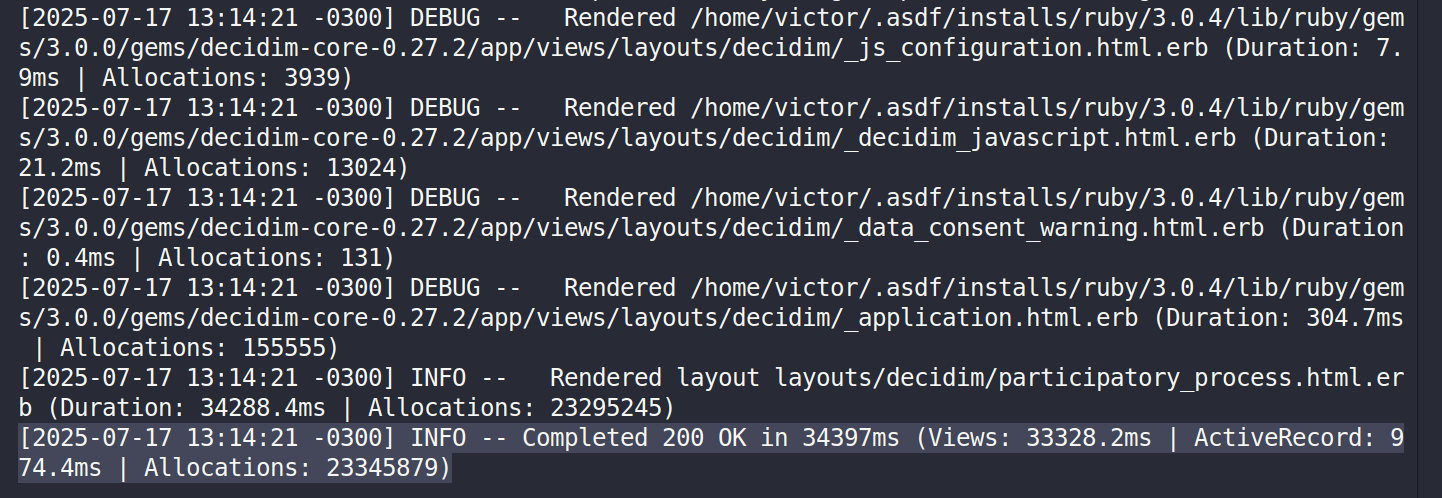
\includegraphics[width=\textwidth]{figuras/analise-log-600-paragrafos.png}
  \fonte{Próprio autor}
\end{figure}

O Decidim possui um mecanismo de representação para UI chamado de \textit{View Models}, também conhecido como \textit{cells}, em português células. Uma célula é um objeto que representa fragmentos da UI, podendo conter desde uma página inteira até um container de comentário ou imagem, por exemplo \cite{decidim-view-models-aka-cells}.

A célula \texttt{ParticipatoryTextProposalCell} é usada para realizar a renderização dos parágrafos do texto participativo. Nessa célula, são utilizados dois arquivos de \textit{view}: \texttt{show.erb} e \texttt{buttons.erb}. Para realizar a renderização de cada parágrafo, o Decidim fará duas chamadas de renderização de \textit{partials}, uma para o arquivo \texttt{show.erb} e outra para o arquivo \texttt{buttons.erb}, que é referenciado pelo arquivo \texttt{show.erb}. Esse comportamento pode ser percebido através do recorte das mensagens de \textit{log} no processamento da requisição, que é mostrado na Figura \ref{fig:logs-partials-show-buttons-evidencia}.

\begin{figure}[htbp]
  \centering
  \caption{Captura de tela dos \textit{logs} evidenciando a utilização de \textit{partials}}
  \label{fig:logs-partials-show-buttons-evidencia}
  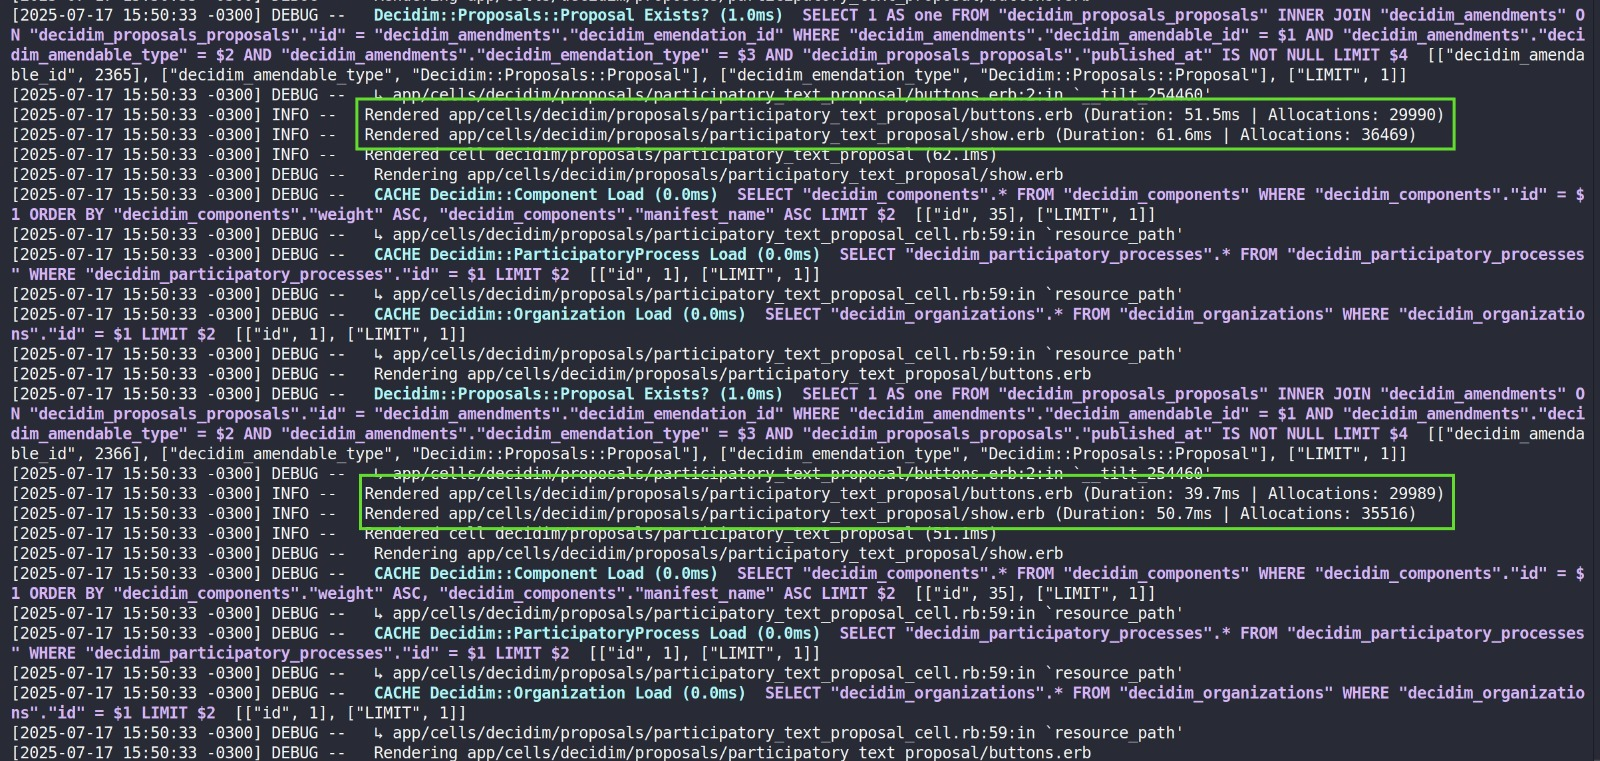
\includegraphics[width=\textwidth]{figuras/logs-partials-show-buttons-evidencia.jpeg}
  \fonte{Próprio autor}
\end{figure}

No repositório oficial do \textit{Ruby on Rails} existe uma \textit{issue} que relata problemas de desempenho com o uso de \textit{partials} em contextos onde há aninhamento, destacando que a renderização de HTML planos acontece com maior agilidade. A \textit{issue} pode ser acessada em \url{https://github.com/rails/rails/issues/41452}.

Dessa forma, a primeira tentativa de ajustes realizada foi a substituição do uso das células na renderização de textos participativos pela renderização \textit{inline} do conteúdo do parágrafo diretamente no arquivo principal da \textit{view}:

\begin{table}[h]
	\begin{tabular}{c}
		\texttt{decidim/proposals/proposals/participatory\_texts/participatory\_text.html.erb}
	\end{tabular}
\end{table}

Após realizar a substituição, foi observado novamente os \textit{logs} do processamento da requisição de renderização da página do texto participativo. O tempo de processamento total da requisição diminuiu de 34.397 milissegundos para 1.139 milissegundos, representando uma redução de 3.019,9\%, e que foi considerada como suficiente para o requisito. Uma captura de tela dos \textit{logs} é exibida na Figura \ref{fig:analise-log-apos-substituicao-celulas}.

Para elucidar a alteração, dado o enfoque deste trabalho na otimização de desempenho, o código fonte será demonstrado em capturas de tela. Contudo, as alterações estão disponíveis no repositório oficial do Brasil Participativo no \textit{Merge Request} em \url{https://gitlab.com/lappis-unb/decidimbr/decidim-govbr/-/merge\_requests/560}.

A versão anterior à modificação pode ser vista na Figura \ref{fig:versao-com-celula}, e a versão ajustada para melhora de desempenho pode ser vista na Figura \ref{fig:versao-inline}.

\begin{figure}[htbp]
  \centering
  \caption{Captura de tela dos \textit{logs} após substituição das células}
  \label{fig:analise-log-apos-substituicao-celulas}
  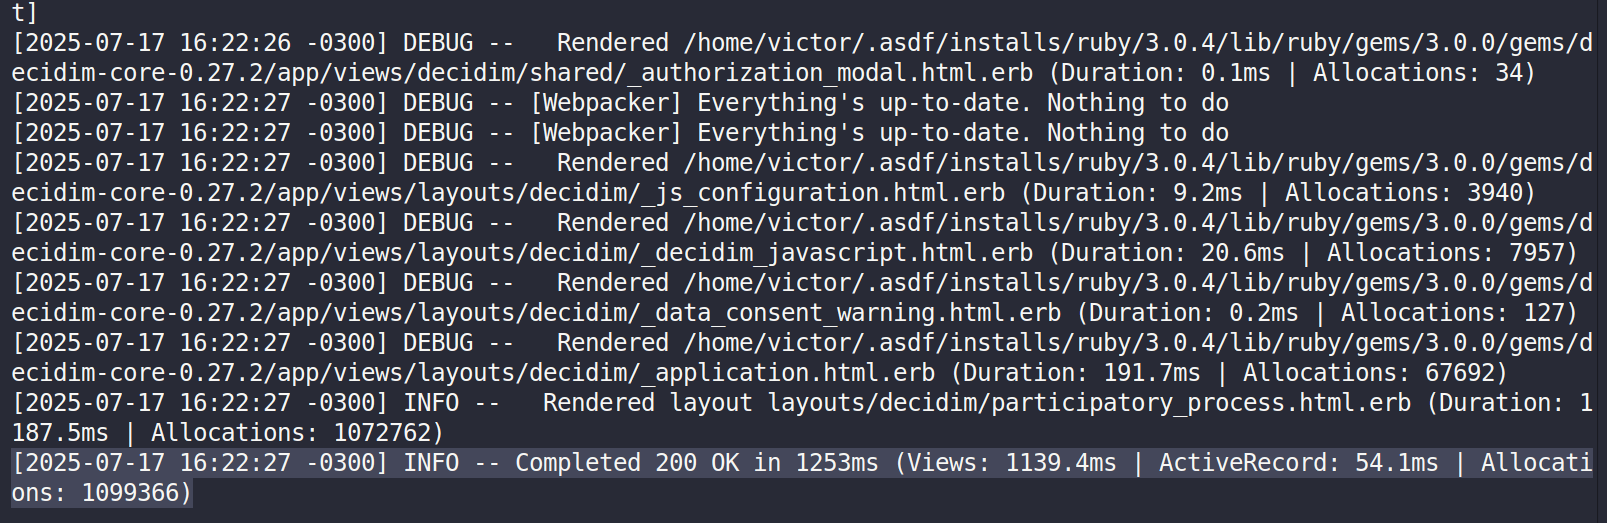
\includegraphics[width=\textwidth]{figuras/analise-log-apos-substituicao-celulas.png}
  \fonte{Próprio autor}
\end{figure}

\begin{figure}[htbp]
  \centering
  \caption{Código fonte da \textit{view} antes da substituição da célula}
  \label{fig:versao-com-celula}
  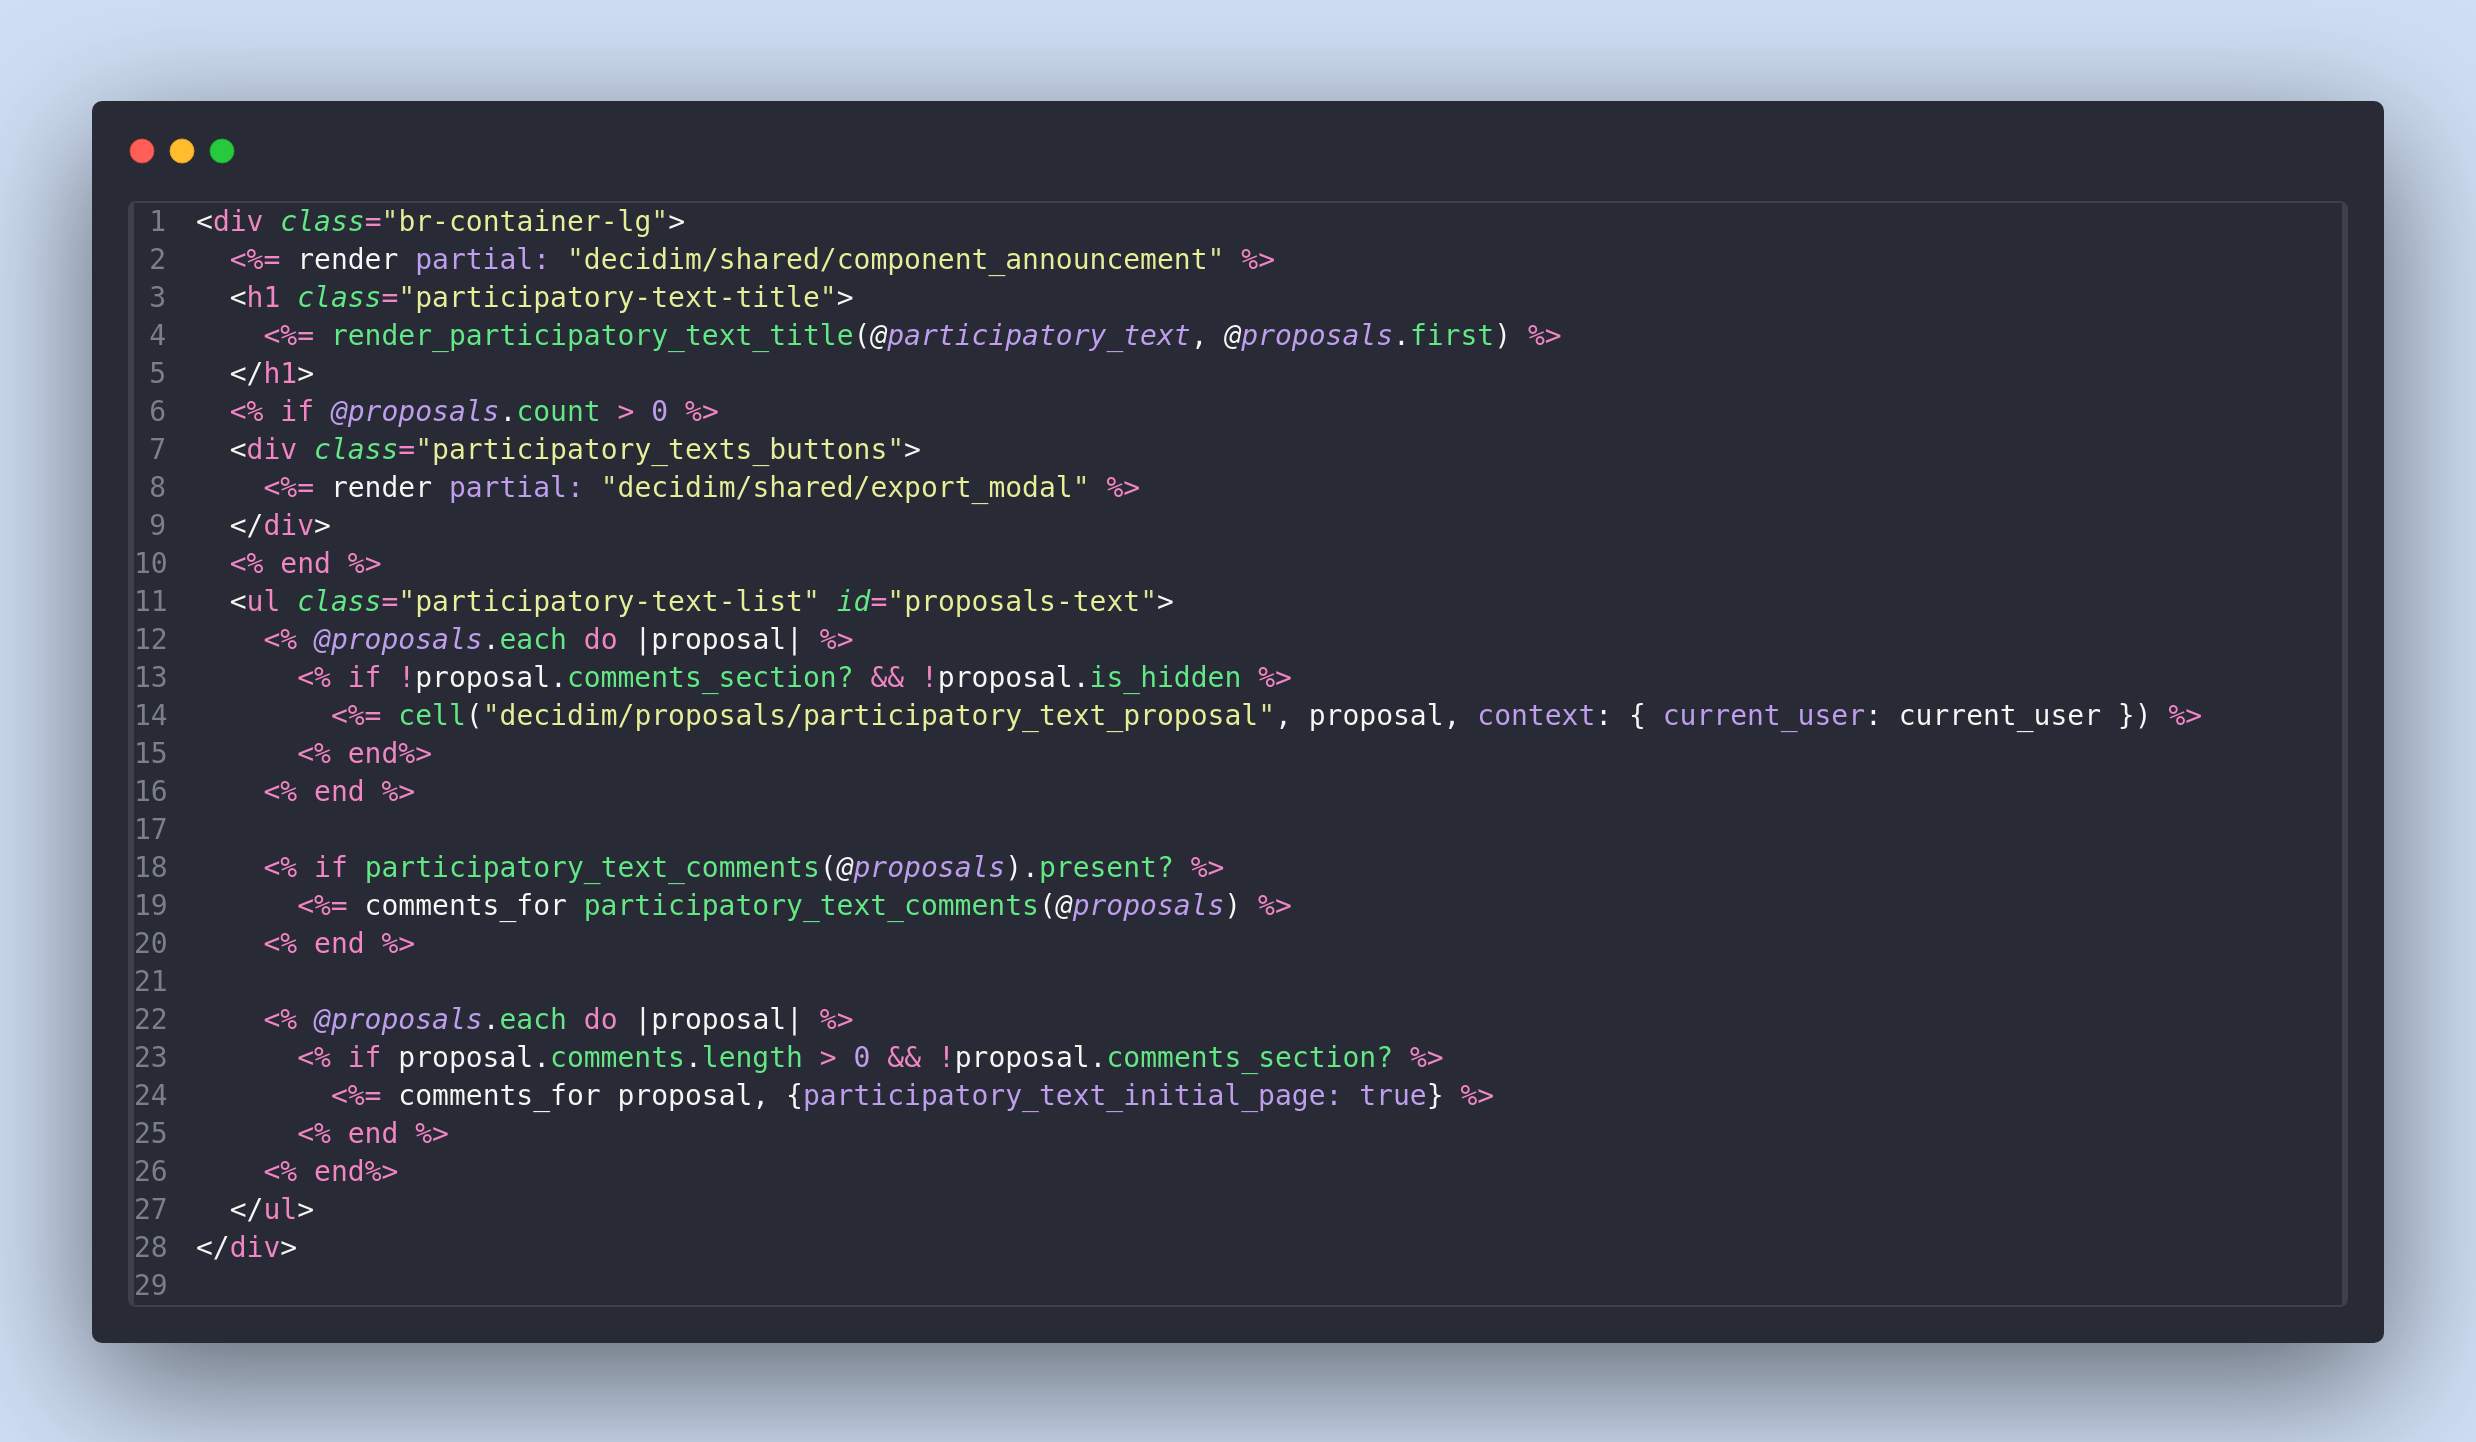
\includegraphics[width=\textwidth]{figuras/versao-celulas-1.png}
  \fonte{Próprio autor}
\end{figure}

\begin{figure}[htbp]
  \centering
  \caption{Código fonte da \textit{view} ajustado para desempenho}
  \label{fig:versao-inline}
  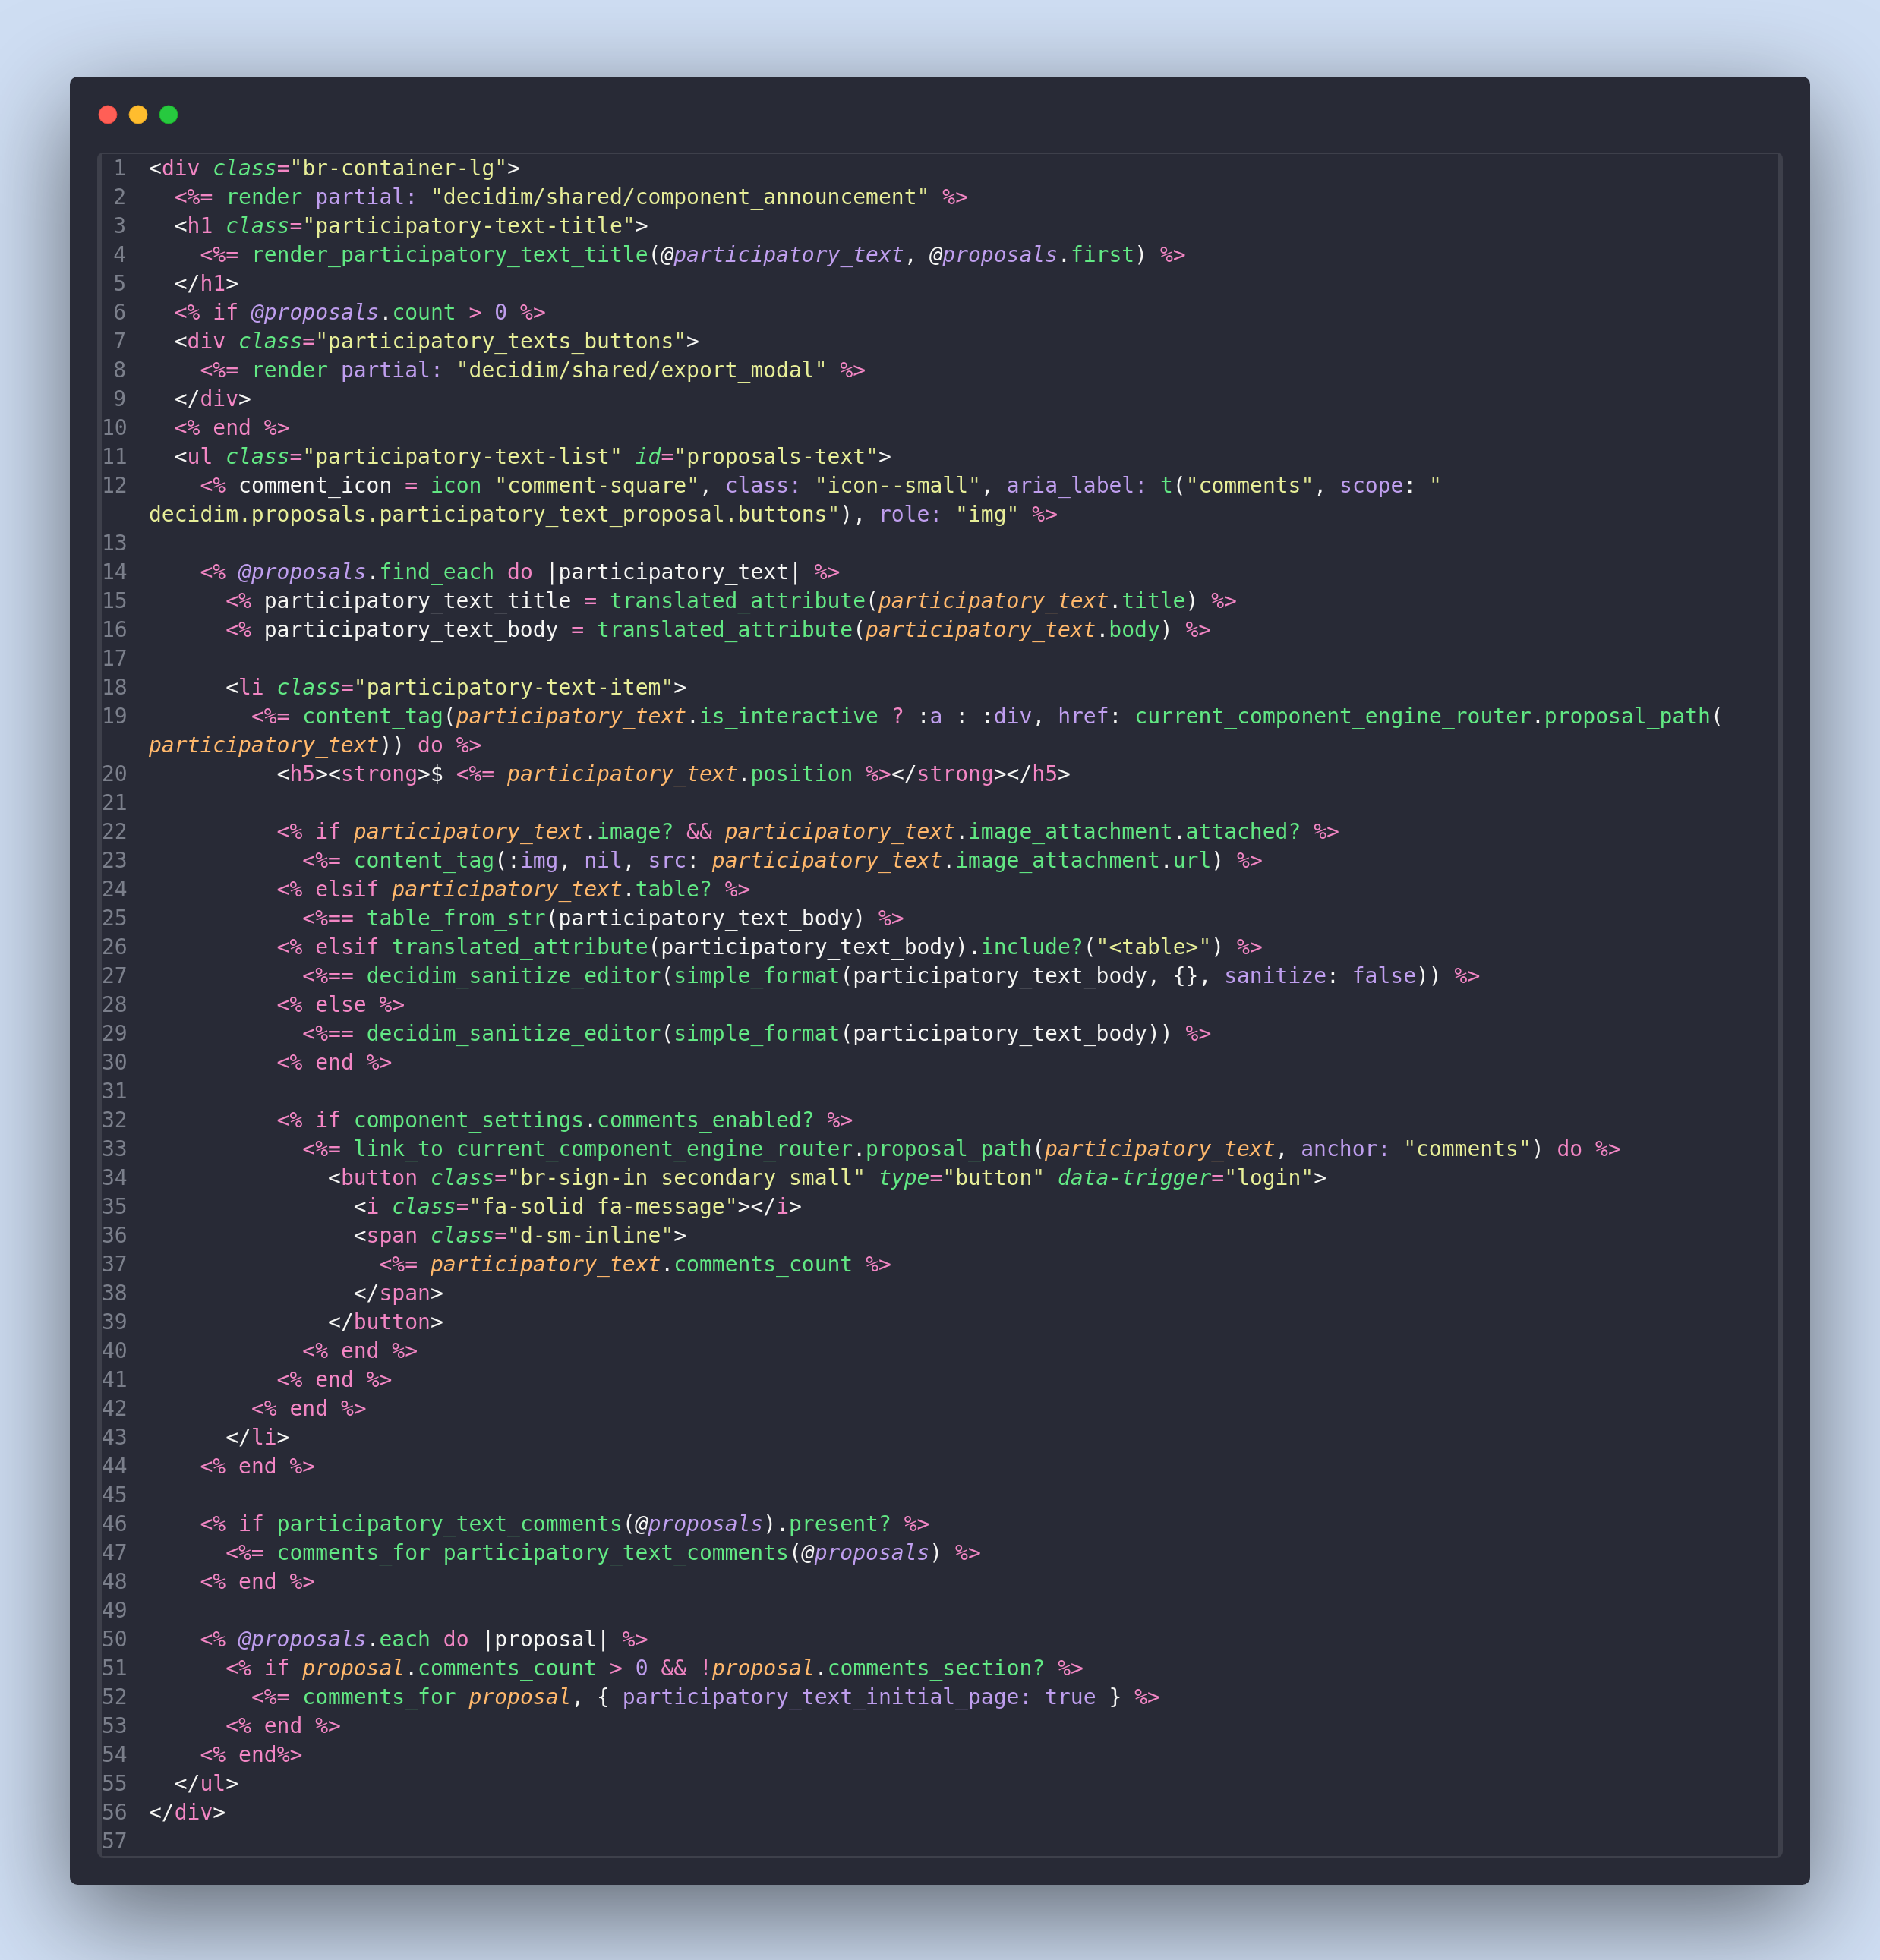
\includegraphics[width=\textwidth]{figuras/versao-inline-1.png}
  \fonte{Próprio autor}
\end{figure}

\subsubsection {Requisito 2 da Sprint 1}

Para cumprir com o segundo requisito, foi adicionado no Brasil Participativo, o editor de textos Trix que é do tipo WYSIWYG. O Trix é um edito de textos pensado para o uso de envio de mensagens, escrita de comentários, artigos e listas. Ele foi criado pela 37signals e está presente em algumas aplicações modernas, como por exemplo o Basecamp, que é uma ferramenta de gestão de projetos também da 37signals. A escolha desse editor de texto se deu pela sua facilidade de integrar com uma aplicação \textit{Rails}, e sua arquitetura baseada em eventos; permitindo com que customizações sejam feitas com pouco código.

Um requisito implícito no requisito 2 era a necessidade de inserir imagens no texto. Por padrão, o Trix posiciona a imagem no texto como um documento "pendente", portanto, é necessário que a aplicação guarde a imagem remotamente e forneça ao Trix um \textit{link} permanente.

Para realizar isso, a \textit{controller} \texttt{Decidim::Govbr::AttachmentsController} foi criada no Brasil Participativo. Esta \textit{controller} possui como papel: receber um arquivo, salvá-lo no \texttt{storage} da aplicação e devolver a URL permanente para aquele arquivo em uma resposta no formato JSON. Essa \textit{controller} ficou expôs a \textit{action} \texttt{create} na rota \texttt{/attachments}. A \textit{action} verifica antes de processar a requisição se o emissor é um usuário logado. O código da \textit{controller} é exibido na Figura \ref{fig:attachments-controller}.

\begin{figure}[htbp]
  \centering
  \caption{Código fonte da \textit{controller} \texttt{Attachments}}
  \label{fig:attachments-controller}
  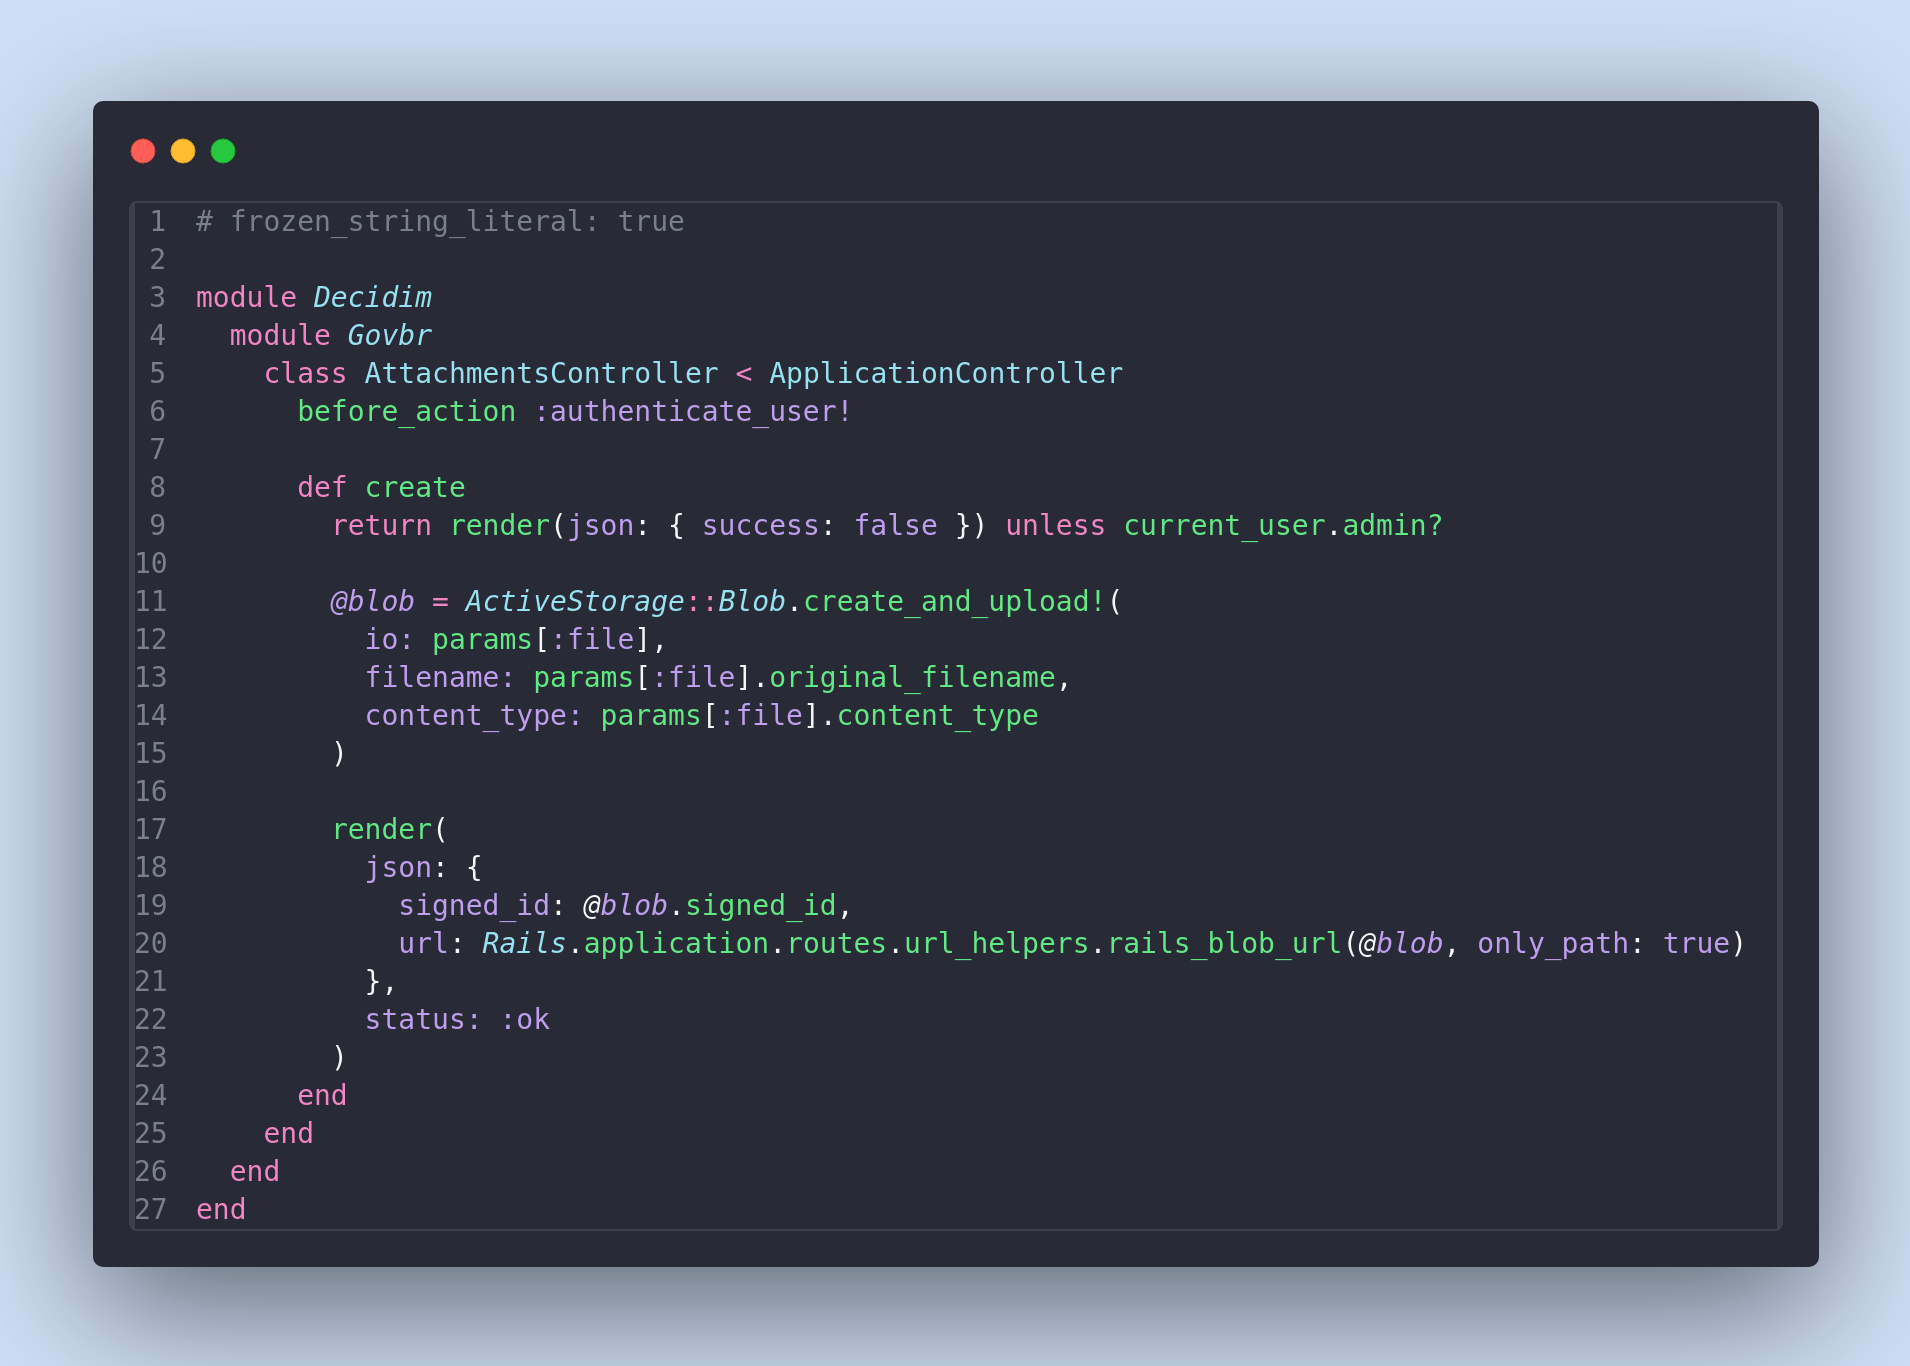
\includegraphics[width=\textwidth]{figuras/attachments-controller.png}
  \fonte{Próprio autor}
\end{figure}

Outro desafio relacionado à inserção do texto através do comando copiar e colar é separar corretamente cada parágrafo de texto. O input do usuário, apesar de parecer apenas texto, na verdade é enviado para o \textit{backend} como uma \texttt{string} HTML, como por exemplo:

\texttt{
<h1>Título do Texto</h1>
<div>
  Parágrafo! Aqui vem o conteúdo do parágrafo do usuário.<br>
  Aqui é outro parágrafo.<br>
</div>
}

Para processar o \textit{input} HTML e transformar em uma estrutura mais flexível de se trabalhar, foi adotada a \textit{gem} Nokogiri. Com o uso do Nokogiri, o texto HTML é transformado em uma estrutura de dados semelhante a uma árvore, onde cada \textit{tag} HTML se torna um nó, com seus elementos filhos, que podem ser outras \textit{tags} ou texto puro, estando disponíveis no atributo \texttt{\#children}.

A fim de separar o texto, depois de realizar o \textit{parsing} do HTML, cada elemento (\textit{tag}) de primeiro nível era considerado um parágrafo. Entretanto, quando o usuário digita um parágrafo e logo em seguida uma quebra de linha para digitar outro parágrafo, o Trix envolvia ambos os parágrafos em uma única \textit{tag} \texttt{<div>}, separando os parágrafos por quebra linha com a \textit{tag} \texttt{<br>}. Para contornar isso, foi adicionada uma verificação no nó, e caso este seja um elemento do tipo \texttt{<div>}, ele não será utilizado como um parágrafo, mas sim os seus elementos filhos diretos, desde que não seja uma \textit{tag} \texttt{<br>}. O código de divisão pode ser conferido na Figura \ref{fig:trix-paragraph-split}.

\begin{figure}[htbp]
  \centering
  \caption{Método para realizar a divisão dos parágrafos do input do usuário}
  \label{fig:trix-paragraph-split}
  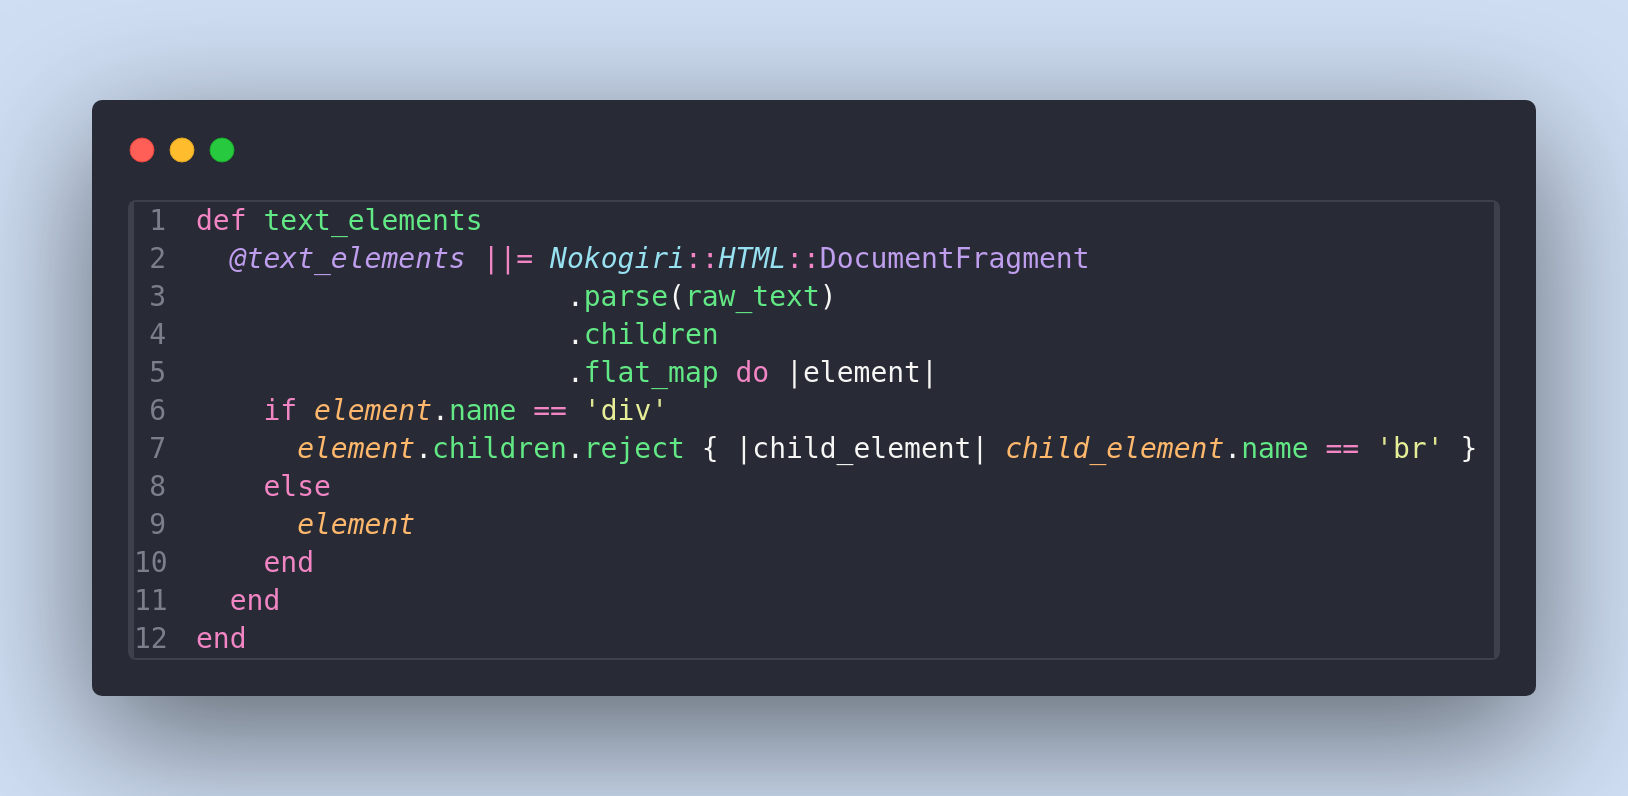
\includegraphics[width=\textwidth]{figuras/trix-paragraph-split.png}
  \fonte{Próprio autor}
\end{figure}

Depois de resolvido o problema de divisão dos parágrafos, havia a gestão das imagens presentes no texto. Dado que cada imagem é enviada para o \texttt{storage} do \textit{Rails} já no momento em que o usuário está digitando o conteúdo do texto no \textit{frontend}, era necessário de alguma maneira saber vincular cada imagem a cada parágrafo.

Um parágrafo na ferramenta de textos participativos é um objeto do tipo \texttt{Proposal}, que também é utilizado para representar propostas na plataforma. No Brasil Participativo, foi feito pela equipe de desenvolvimento do Lab Livre uma customização que permite que cada proposta tenha relacionamento com nenhum ou vários arquivos. Sendo assim, uma das etapas de pré-processamento do \textit{input} é descobrir as imagens que já estão no \texttt{storage} do \textit{Rails} e vinculá-las a cada proposta (parágrafo).

A primeira etapa é feita através da extração do atributo \texttt{signed\_id} dos nós Nokogiri que são do tipo \texttt{figure}. Na integração de envio de arquivos do Trix para o \texttt{storage} do \textit{Rails}, além da URL da imagem, a \textit{controller} \texttt{Attachments} envia o atributo \texttt{signed\_id}, que funciona como um identificador para o arquivo. Esse atributo é vinculado ao elemento de imagem do Trix, e fica disponível no atributo \texttt{data-trix-attachment}.

Depois de extrair o \texttt{signed\_id}, a próxima etapa é a criação de fato dos parágrafos. Como dito, cada parágrafo é salvo em um objeto do tipo \texttt{Proposal}. Nesse momento o parágrafo é salvo podendo seu tipo ser:

\begin{itemize}
	\item Título (enumerador \texttt{section}), caso seja \texttt{<h1>};
	\item Sub-título (enumerador \texttt{sub\_section}), caso seja \texttt{<h2>} e \texttt{<h3>};
	\item Imagem (enumerador \texttt{image}), caso seja \texttt{<figure>};
	\item Artigo (enumerador \texttt{article}), caso seja qualquer outra \textit{tag} HTML.
\end{itemize}

Caso o parágrafo seja do tipo imagem, o atributo \texttt{signed\_id} é usado para localizar o arquivo no \texttt{storage} e realizar o vinculo.

\subsubsection {Requisito 3 da Sprint 1}

A refatoração da página de visualização do rascunho, que é a página utilizada para fazer edições no texto submetido, tinha como propósito ser o mais parecida quanto possível com a tela de visualização do texto já publicado. Segundo o time de produto do Lab Livre, esta abordagem traria melhor experiência ao usuário administrador, que no momento da edição do rascunho teria ideia de como o texto se pareceria com o que o usuário vê.

Sendo assim, a primeira ideia foi a de extrair o padrão visual da \textit{view} utilizada na renderização do texto, e utilizá-la em outra página dedicada para a edição do texto. Ora, o Decidim segmenta o sistema em três contextos diferentes: o \texttt{system admin}, \texttt{admin} e \texttt{public}, cada um deles tem o seu próprio \texttt{namespace} dentro do código-fonte, fazendo uma separação entre os estilos, permissionamentos, \textit{views} e \textit{controllers}.

A página de visualização do texto fica no contexto \texttt{public}, equanto a página de edição do texto fica no contexto \texttt{admin}. Para que a transição entre a edição e a visualização do texto fosse irrisória, uma das decisões foi a de implementar a página de edição refatorada no contexto \texttt{public}. Dessa maneira, o \textit{layout} e a lógica de renderização dos parágrafos, já com a otimização de desempenho, foi separada em uma \textit{partial}, que é renderizada tanto pela página de visualização quanto pela de edição.

A \textit{partial} criada (\texttt{\_lightweight\_text\_render.html.erb}) faz verificações sobre o estado do texto, e o usuário que a está acessando. Caso o usuário seja um administrador e o texto ainda não tenha sido publicado, botões de ações aparecerão para manipular o texto. A página de edição do texto com os seus botões de ação pode ser vista na Figura \ref{fig:edicao-texto-v1}.

\begin{figure}[htbp]
  \centering
  \caption{Tela de edição de textos refatorada para o escopo \texttt{public}}
  \label{fig:edicao-texto-v1}
  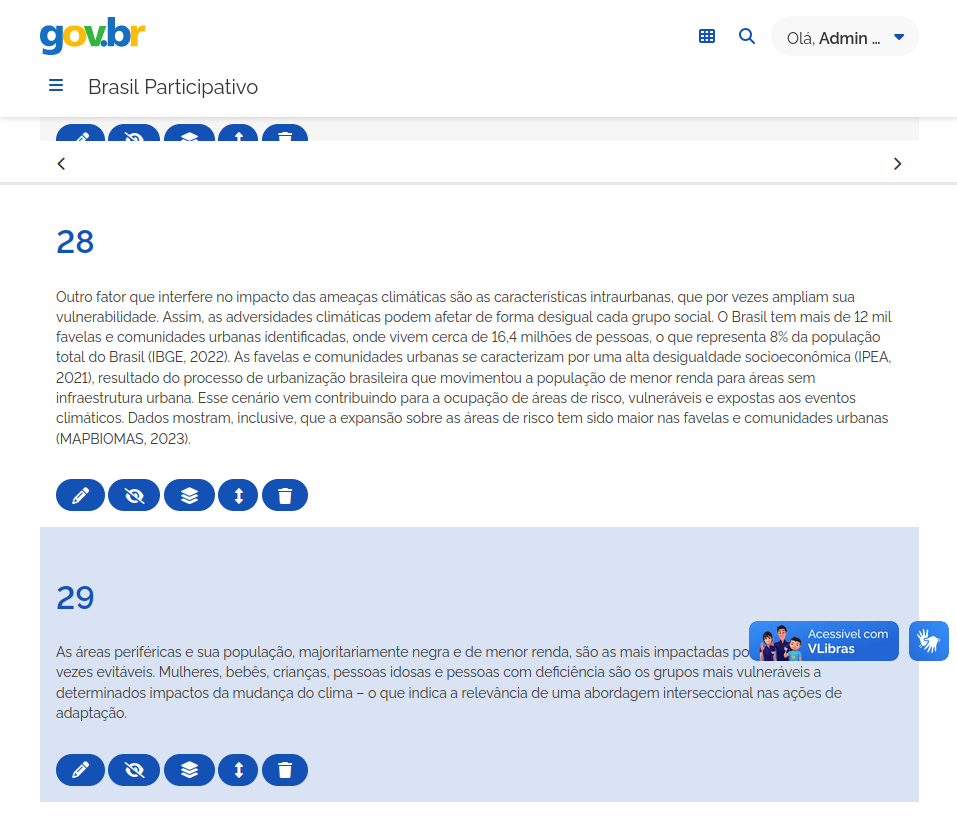
\includegraphics[width=\textwidth]{figuras/edicao-texto-v1.png}
  \fonte{Próprio autor}
\end{figure}

A página de edição conta com cinco ações possíveis:

\begin{itemize}
	\item Editar conteúdo do texto;
	\item Ocultar parágrafo;
	\item Mesclar parágrafos;
	\item Move parágrafo;
	\item Remover parágrafo.
\end{itemize}

O \textit{Merge request} contendo as alterações descritas acima pode ser encontrado em \url{https://gitlab.com/lappis-unb/decidimbr/decidim-govbr/-/merge_requests/561}.

\subsection {Sprint 2}

A \textit{sprint} 2 foi caracterizada pela correção de comportamentos inesperados que surgiram durante os testes de aceitação conduzido pelo time de produto, além de outros ajustes. Os trabalhos começaram assim que a lista de ajustes necessários foi levantada, e pode ser sumarizada nos seguintes requisitos:

\begin{itemize}
	\item \textbf{Requisito 1 da Sprint 2}: Corrigir problema onde um parágrafo que possua trechos em itálico e negrito são erroneamente divididos em mais de um parágrafo;
	\item \textbf{Requisito 2 da Sprint 2}: Corrigir problema de imagens quebradas quando copiadas do Google Docs ou Microsft Word;
\end{itemize}

\subsubsection {Requisito 1 da Sprint 2}

Alguns parágrafos que possuiam itálico e negrito em seu conteúdo, eram erroneamente divididos em multiplos parágrafos. Por exemplo o \textit{input} HTML:

\begin{table}[h]
	\begin{tabular}{c}
		\texttt{<h1>Título do Texto</h1>}\\
		\texttt{<div>}\\
			\texttt{Parágrafo! <strong>Aqui vem o conteúdo</strong>}\\
			\texttt{do parágrafo do usuário.<br>}\\
			\texttt{Aqui é outro parágrafo.<br>}\\
		\texttt{</div>}\\
	\end{tabular}
\end{table}

seria dividido em cinco parágrafos:

\begin{itemize}
	\item \texttt{<h1>Título do Texto</h1>};
	\item \texttt{Parágrafo!};
	\item \texttt{<strong>Aqui vem o conteúdo</strong>};
	\item \texttt{do parágrafo do usuário.};
	\item \texttt{Aqui é outro parágrafo.}.
\end{itemize}

Isso acontece devido ao fato de que no Nokogiri, texto puro também é tratado como um nó na árvore do documento XML/HTML. Ao fazer a tratativa de separar as \texttt{<div>} exibida na Figura \ref{fig:trix-paragraph-split}, o método \texttt{\#children} separará o primeiro parágrafo em três, pois entende-se que a \textit{tag} \texttt{strong} é um elemento independente na árvore. A Figura \ref{fig:arvore-nokogiri-problema-italico-negrito} ilustra o comportamento.

\begin{figure}[htbp]
  \centering
  \caption{Diagrama representando a árvore do HTML após o \textit{parsing} do Nokogiri}
  \label{fig:arvore-nokogiri-problema-italico-negrito}
  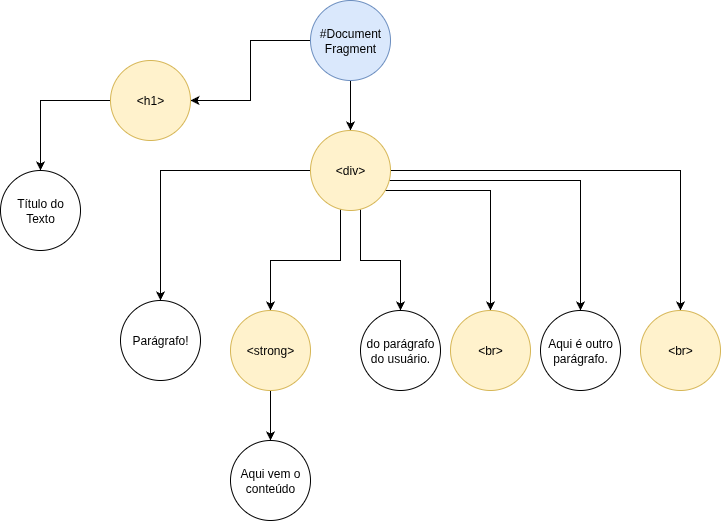
\includegraphics[width=\textwidth]{figuras/arvore-nokogiri-problema-italico-negrito.png}
  \fonte{Próprio autor}
\end{figure}

Para resolver esse problema, foi criado um método para fazer a extração dos parágrafos com base nos filhos diretos de uma \texttt{<div>}, onde dois ou mais filhos podem ser considerados pertencentes ao mesmo parágrafo. O critério para dividir os nós filhos entre mais de um parágrafo é o aparecimento de um elemento \texttt{<br>} entre eles. A Figura \ref{fig:diagrama-metodo-split-nokogiri} mostra como a divisão ocorre na visualização de árvore. Caso seja encontrado um elemento \texttt{<div>}, seus filhos serão agrupados até que se encontre o elemento divisor (\texttt{<br>}). Os elementos são analisados da esquerda para direita. Esse método foi inserido diretamente na classe \texttt{Nokogiri::XML::Nodeset} na inicialização da aplicação. A Figura \ref{fig:metodo-split-nokogiri} mostra a implementação e o uso.

\begin{figure}[htbp]
  \centering
  \caption{Diagrama representando o agrupamento de elementos filhos separados por \texttt{<br>}}
  \label{fig:diagrama-metodo-split-nokogiri}
  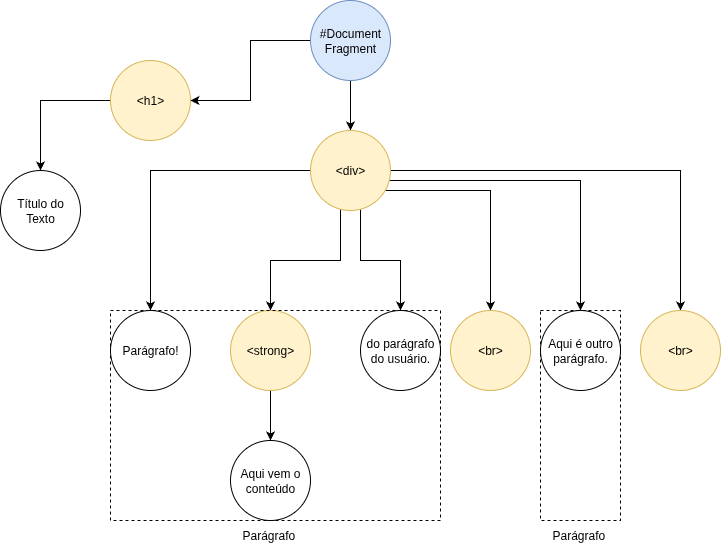
\includegraphics[width=\textwidth]{figuras/diagrama-metodo-split-nokogiri.png}
  \fonte{Próprio autor}
\end{figure}

\begin{figure}[htbp]
  \centering
  \caption{Definição e uso do método \texttt{split}}
  \label{fig:metodo-split-nokogiri}
  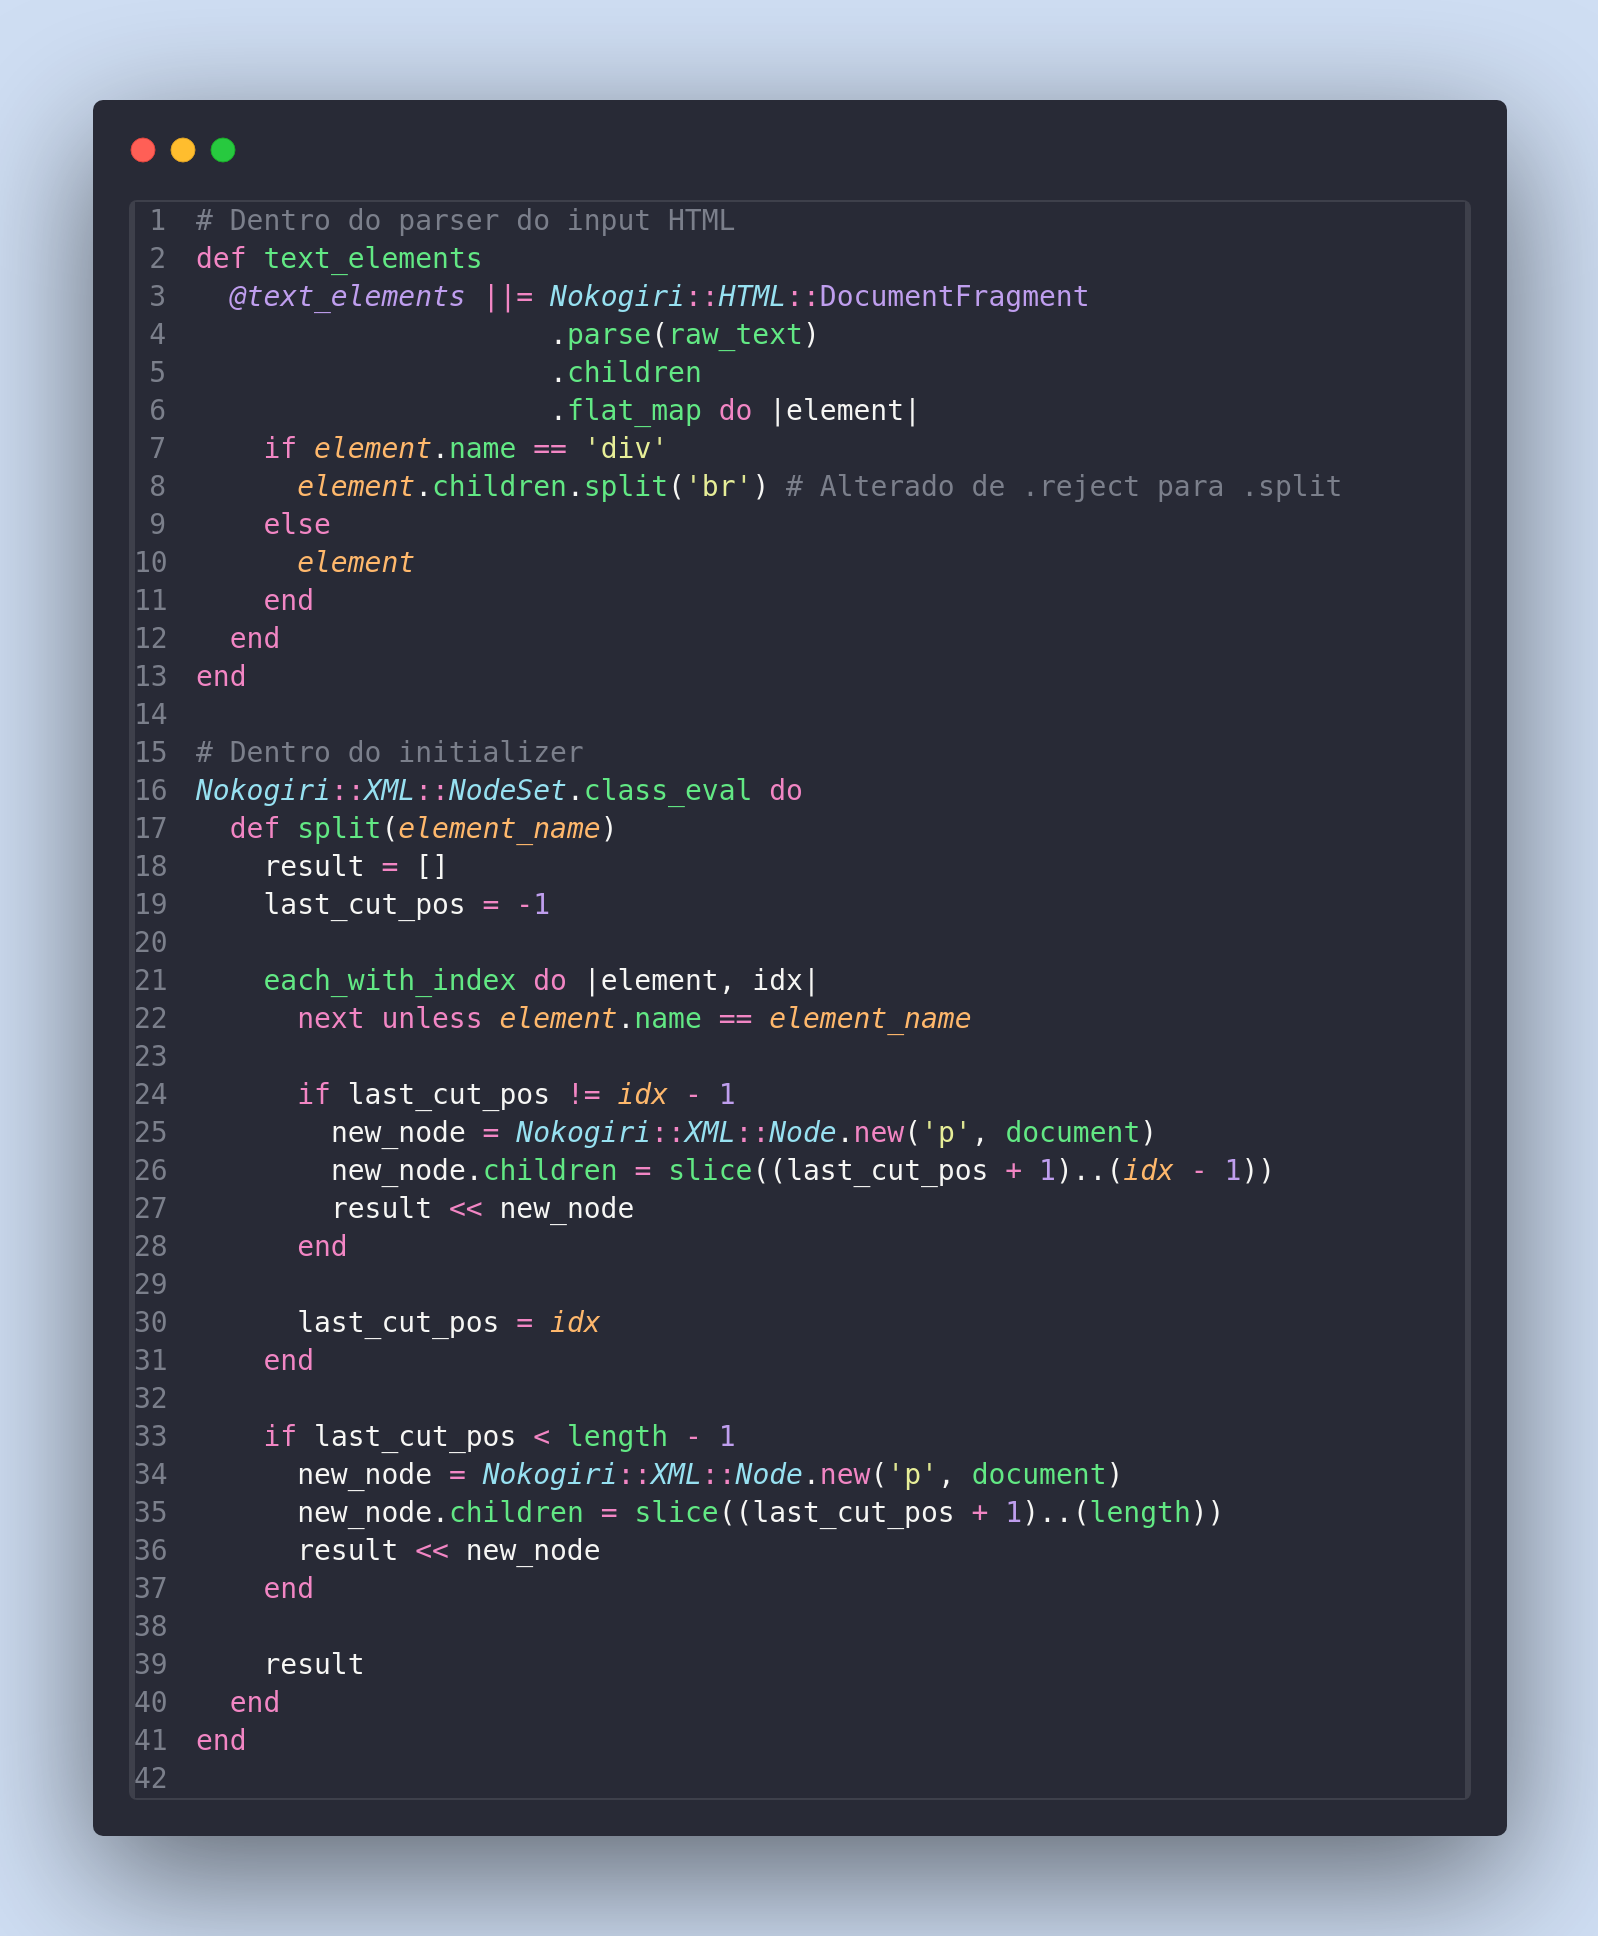
\includegraphics[width=\textwidth]{figuras/metodo-split-nokogiri.png}
  \fonte{Próprio autor}
\end{figure}

\subsubsection {Requisito 2 da Sprint 2}

Ao utilizar o comando copiar e colar em editores de texto como o Google, na maioria das vezes o conteúdo da imagem em si não era copiado, mas sim um \textit{link} para onde está guardada. Para esses casos, a imagem (\texttt{<img>}) já era inserida no texto com o seu atributo \texttt{src} preenchido, e não era automaticamente enviada para o \texttt{storage} do \textit{Rails}, pois o seu conteúdo sequer estava lá.

Para resolver esse problema, uma das possibilidades seria fazer uma requisição para a fonte da  para em seguida enviá-la para o \texttt{storage} usando a \textit{controller} \texttt{Attachments}. Mas, essa alternativa tinha dois problemas: problemas com \textit{Cross-Origin Resource Sharing} (CORS), e disponibilidade limitada do recurso.

CORS é um mecanismo para controle de requisições entre domínios distintos quando a requisição é feita pelo \textit{browser}, fazendo com que nem sempre o Brasil Participativo tenha permissão para baixar imagens de outras fontes automaticamente \cite{cors-explanation}.

Outra possibilidade seria deixar o elemento HTML que representa a imagem intocado e referenciando o \textit{link} externo, porém, algumas fontes possuem mecanimos de \textit{throttle} para impedir que uma determinada origem faça requisições demais, além de que não há garantias de que o recurso estará disponível a qualquer instante que se queira buscá-lo.

Portanto, para garantir a consistência na inserção de imagens no texto, o usuário não conseguirá mais inserir imagens através do comando copiar e colar. Será necessário manualmente baixar a imagem no computador e inserí-la no corpo do texto, seja arrastando, seja utilizando a funcionalidade de upload de arquivos do Trix.

Para realizar esse comportamento, foi escrito uma nova customização no Trix para observar o evento \texttt{trix-before-paste}, que é disparado antes do conteúdo ser inserido no \textit{input}. Caso seja detectado algum elemento de imagem no conteúdo colado, este será substituído por uma mensagem de aviso, além de alertar o usuário com uma mensagem do próprio navegador de que ele deve seguir outro procedimento para realizar a inserção daquela imagem. Na Figura \ref{fig:trix-removendo-imagens} é exibido o código JavaScript que realiza essa verificação.

\begin{figure}[htbp]
  \centering
  \caption{Código JavaScript para remover imagens inseridas através do copiar e colar}
  \label{fig:trix-removendo-imagens}
  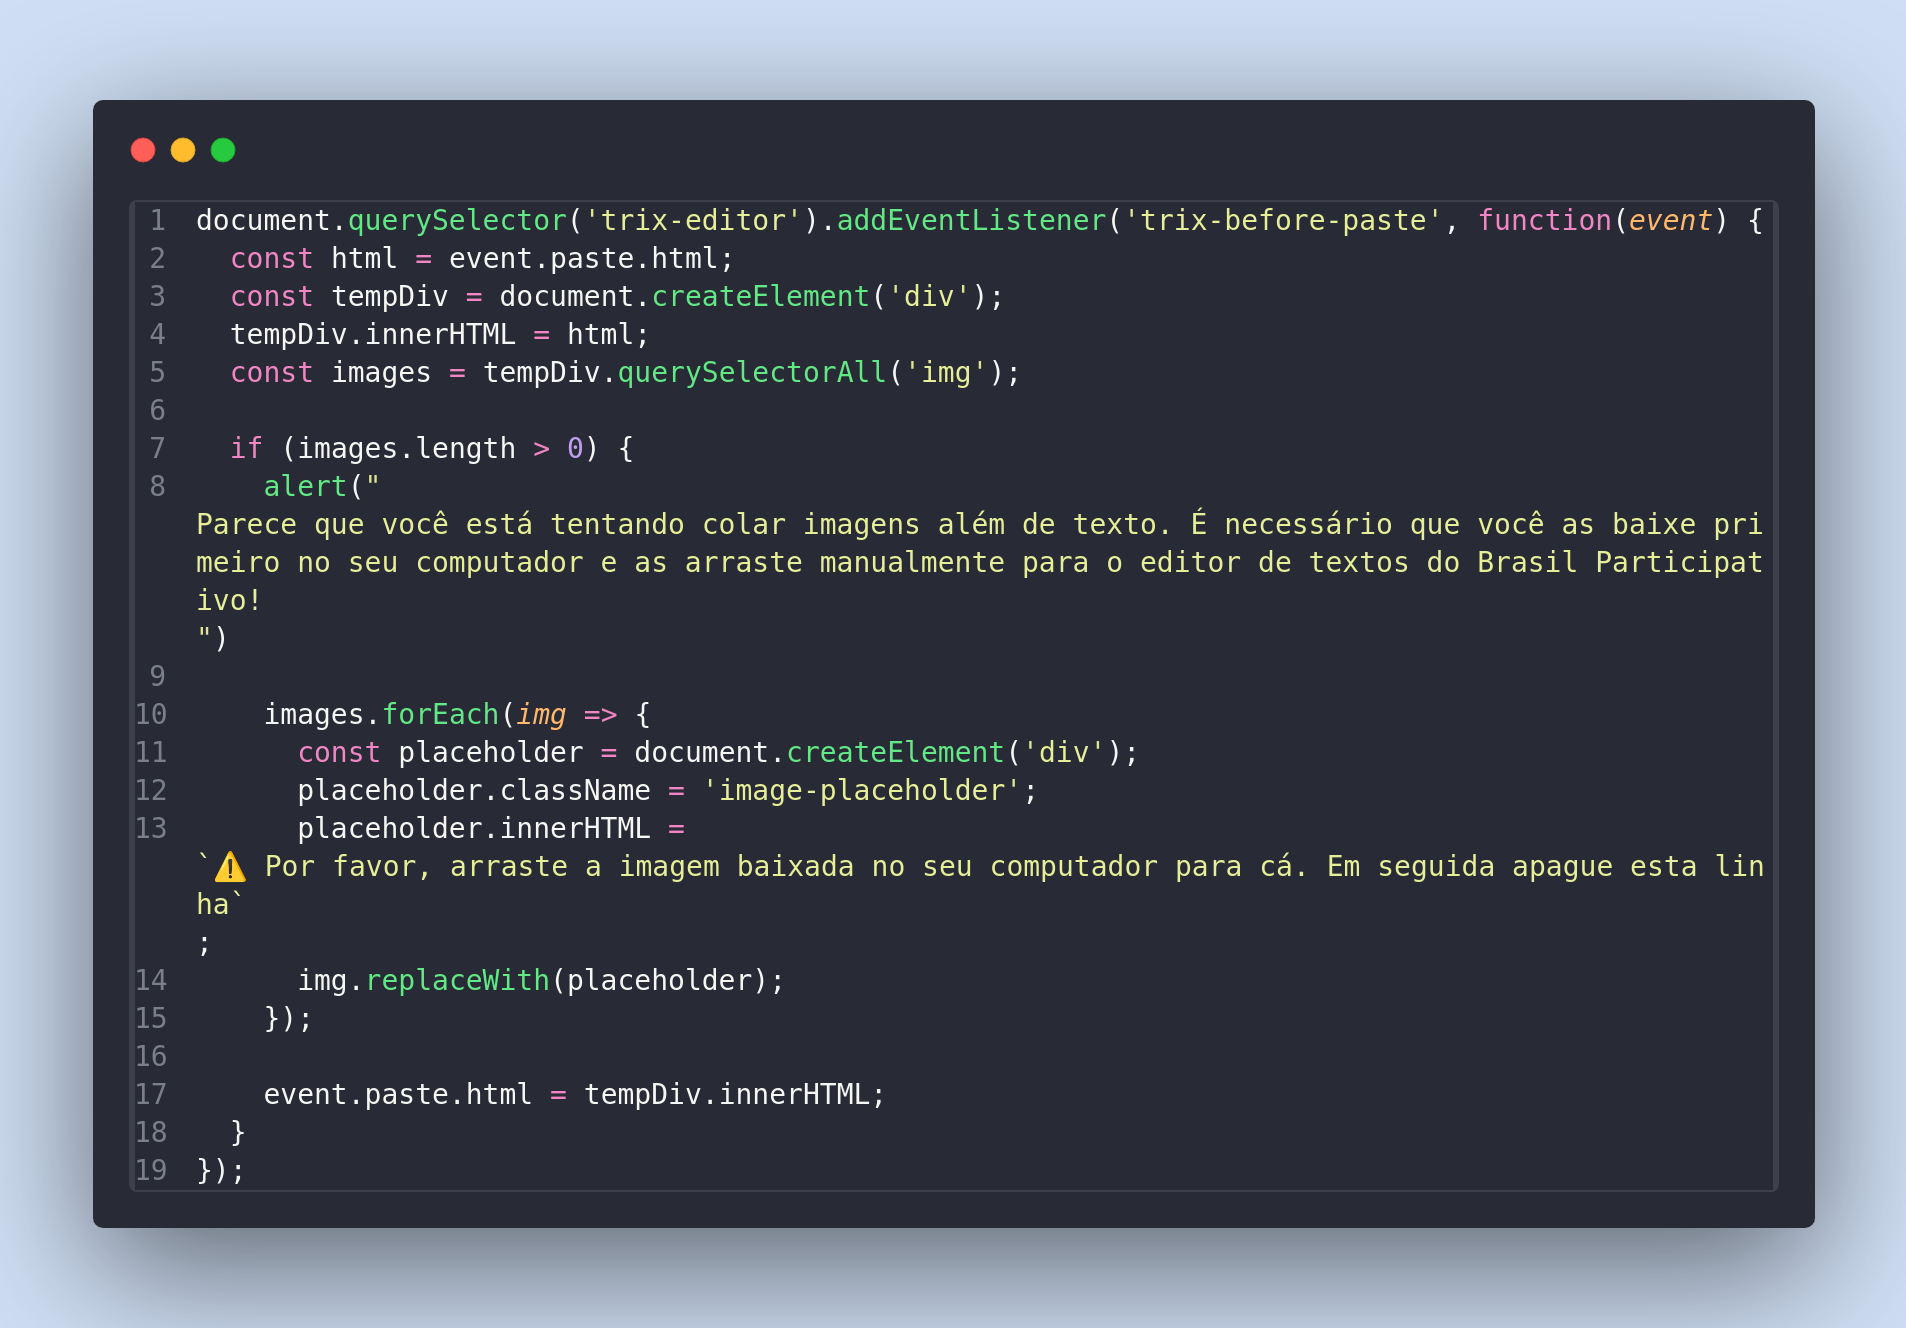
\includegraphics[width=\textwidth]{figuras/trix-removendo-imagens.png}
  \fonte{Próprio autor}
\end{figure}

\subsection {Sprint 3}

Design, UX, UI, flow

\subsection {Sprint 4}

Após todos os ajustes já realizados no \textit{frontend} para se adequar aos padrões visuais expostos no protótipo feito pelo time de \textit{design} do Lab Livre, a quarta \textit{sprint} foi caracaterizada por um único requisito: ter tabelas no texto. No respositório oficial do Trix de textos há uma \textit{issue}, já fechada, onde usuários questionam se há planos de adicionar o suporte a tabelas; até a data deste trabalho não houve indícios de que mantenedores do projeto irão atuar nessa demanda. A \textit{issue} mencionada pode ser acessada em \url{https://github.com/basecamp/trix/issues/539}.

\subsubsection {Requisito 1 da Sprint 4}

Dada a limitação do Trix em relação ao uso de tabelas, anteriormente foi acordado com o time de produto do Lab Livre que estas seriam inseridas no texto no formato de imagens. Entretanto, em reuniões de \textit{feedback} com os \textit{stakeholders}, viu-se que era impraticável em termos de experiência do usuário e usabilidade proceder dessa maneira.
Foram feitas reuniões de descorberta com o time responsável pela plataforma Participa+ Brasil, onde existe funcionalidade semelhante ao texto participativo, e que existe o suporte a tabelas. Como saída dessa reunião foram sugeridos alguns editores de texto, dentre eles: Jodit, CKEditor 5 e o TinyMCE. No Participa+ Brasil é utilizado o editor Jodit.

Com base na premissa de que alguns usuários poderiam migrar do Participa+ Brasil para o Brasil Participativo, o Jodit foi escolhido como potencial escolha. Para garantir que haveria compatibilidade com a ferramenta de textos do Brasil Participativo, foi realizado um teste localmente, trocando o Trix pelo Jodit na página de inserção de conteúdo para criação de texto participativo.
O teste foi realizado inserindo na própria \textit{view} da página \textit{links} para o JavaScript e o CSS do Jodit, conforme descrito na própria documentação do editor. Para validar a viabilidade de uso do editor, foram feitas várias provas inserindo tabelas, imagens e textos formatados através do comando de copiar e colar, todos os textos vindo do Google Docs, Microsoft Word e LibreOffice Writer. Foram manualmente persistidos alguns parágrafos que continham tabelas, e posteriormente exibidos com sucesso na tela de visualização do texto participativo.

Com o sucesso desses testes, o desenvolvimento finalmente seguiria com foco total na implantação do Jodit no Brasil Participativo. Como próximo passo era preciso, da mesma forma como foi feito para o Trix, achar formas de persistir as imagens, inseridas no editor, no \texttt{storage}. O Jodit possui a opção \texttt{uploader.insertImageAsBase64}, que guarda o conteúdo da imagem no formato de Data URL na própria estrutura do HTML.
Data URL é uma maneira de embutir o conteúdo de arquivo de forma \textit{inline} em documentos \cite{data-urls-mdn}. O atributo \texttt{src} de \textit{tags} \texttt{<img>} é preenchido com o próprio conteúdo da imagem codificado em Base64, ao invés de ter um \textit{link} para onde esta estaria guardada. Dessa maneira, ao invés de tentar guardar a imagem no \texttt{storage} logo que for inserida no texto, pode-se guardar a imagem apenas quando o usuário submeter o texto para ser criado.
Na forma como era feita com o Trix, caso o usuário arrastasse uma imagem para o texto e depois a removesse antes mesmo de submeter o texto, esta ficaria sem qualquer uso, e mesmo assim continuaria persistida no \texttt{storage}. Com o uso de Data URLs, é possível evitar esses casos e ter maior controle do ciclo de vida das imagens.

O próximo passo seria, então, fazer o \textit{parsing} do \textit{input} HTML e realizar a divisão dos parágrafos. Diferentemente do Trix que por padrão inseria novos paragrafos envoltos de \textit{tags} \texttt{<div>}, da forma como foi configurado, no Jodit os parágrafos são envoltos de \textit{tags} \texttt{<p>}, e a cada quebra de linha uma nova \textit{tags} \texttt{<p>} é criada para servir de container para o texto.
O único problema é a formatação de alguns textos quando copiados do Google Docs e do Microsft Word. Alguns utilizam \textit{tags} \texttt{<p>} para servir de container para \textit{tags} \texttt{<img>}, além de em alguns momentos o texto de vários parágrafos estar envolto de uma única \textit{tag} \texttt{<strong>}. Esse comportamento foi classificado neste trabalho como "\textit{tags} modificadoras de texto sendo utilizadas como \texttt{<div>}", e guiou o desenvolvimento do \textit{parser} para suportar a migração para o Jodit.

A versão final do \textit{parser} de textos participativos executa três passos:

\begin{enumerate}
	\item Substituir sequência de caracteres de espaço em branco ou não imprimíveis por um único espaço no \textit{input} HTML ainda em formato \texttt{string};
	\item Realizar a transformação para a estrutura do Nokogiri;
	\item Separar parágrafos removendo aqueles que estivem em branco.
\end{enumerate}

A figura \ref{fig:jodit-parser-final} demonstra o código fonte da etapa de \textit{parsing} do \textit{input}.

\begin{figure}[htbp]
  \centering
  \caption{Código fonte da função que realiza o \textit{parsing} do HTML vindo do Jodit}
  \label{fig:jodit-parser-final}
  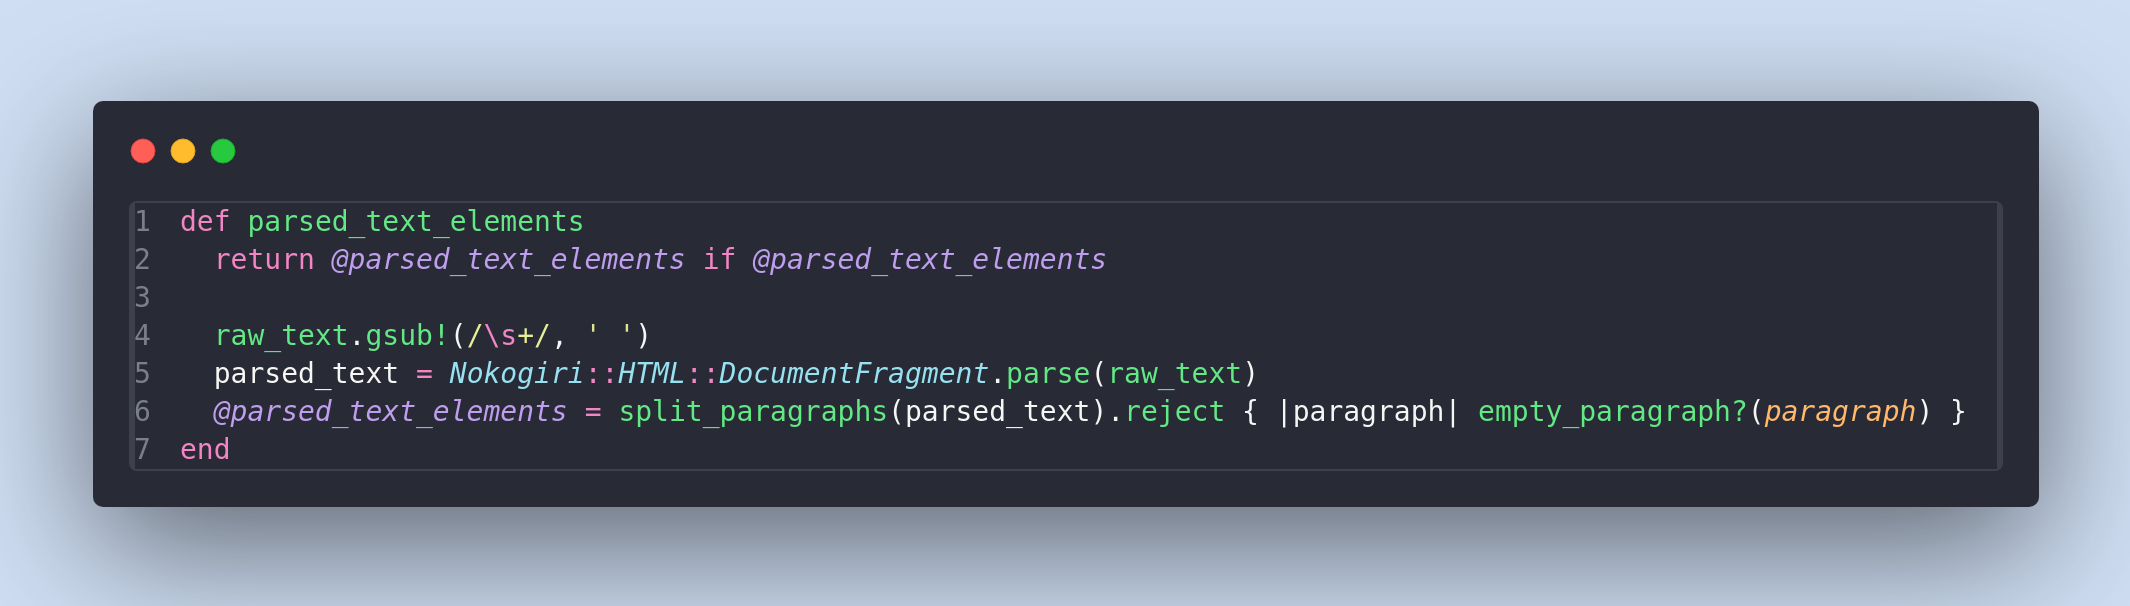
\includegraphics[width=\textwidth]{figuras/jodit-parser-final.png}
  \fonte{Próprio autor}
\end{figure}

O método \texttt{split\_paragraphs} é um método também criado a mão para satisfazer os casos de bordas classificados como "\textit{tags} modificadoras de texto sendo utilizadas como \texttt{<div>}". Para resolver esse problema, foi utilizada uma estratégia recursiva para percorrer a árvore de nós do Nokogiri e determinar quais nós pertencem ao mesmo parágrafo ou não.

A verificação começa no nó raiz, que é o próprio \texttt{DocumentFragment}. Se o nó que está sendo avaliado nesse momento for uma \texttt{<div>} ou o \texttt{DocumentFragment}, recursivamente chama a verificação para todos os seus nós filhos retornados pelo método \texttt{children}, pegando o resultado e compilando em um \texttt{Array} achatado, isto é, um \texttt{Array} que não possui elementos do tipo \texttt{Array} dentro de si. A mesma coisa também é feita caso o nó seja um modificador de texto sendo usado como \texttt{<div>}. Caso contrário, é retornado um \texttt{Array} envolvendo o próprio nó apenas. A ideia central por trás desse algoritmo é a de eliminar elementos que sejam uma \texttt{<div>} ou que ajam como uma \texttt{<div>}, e escolher ramos da árvore para serem parágrafos. O código fonte dessa verificação pode ser visto na Figura \ref{fig:split-paragraphs-jodit}.

\begin{figure}[htbp]
  \centering
  \caption{Código fonte do método que realiza a divisão de parágrafos do Jodit}
  \label{fig:split-paragraphs-jodit}
  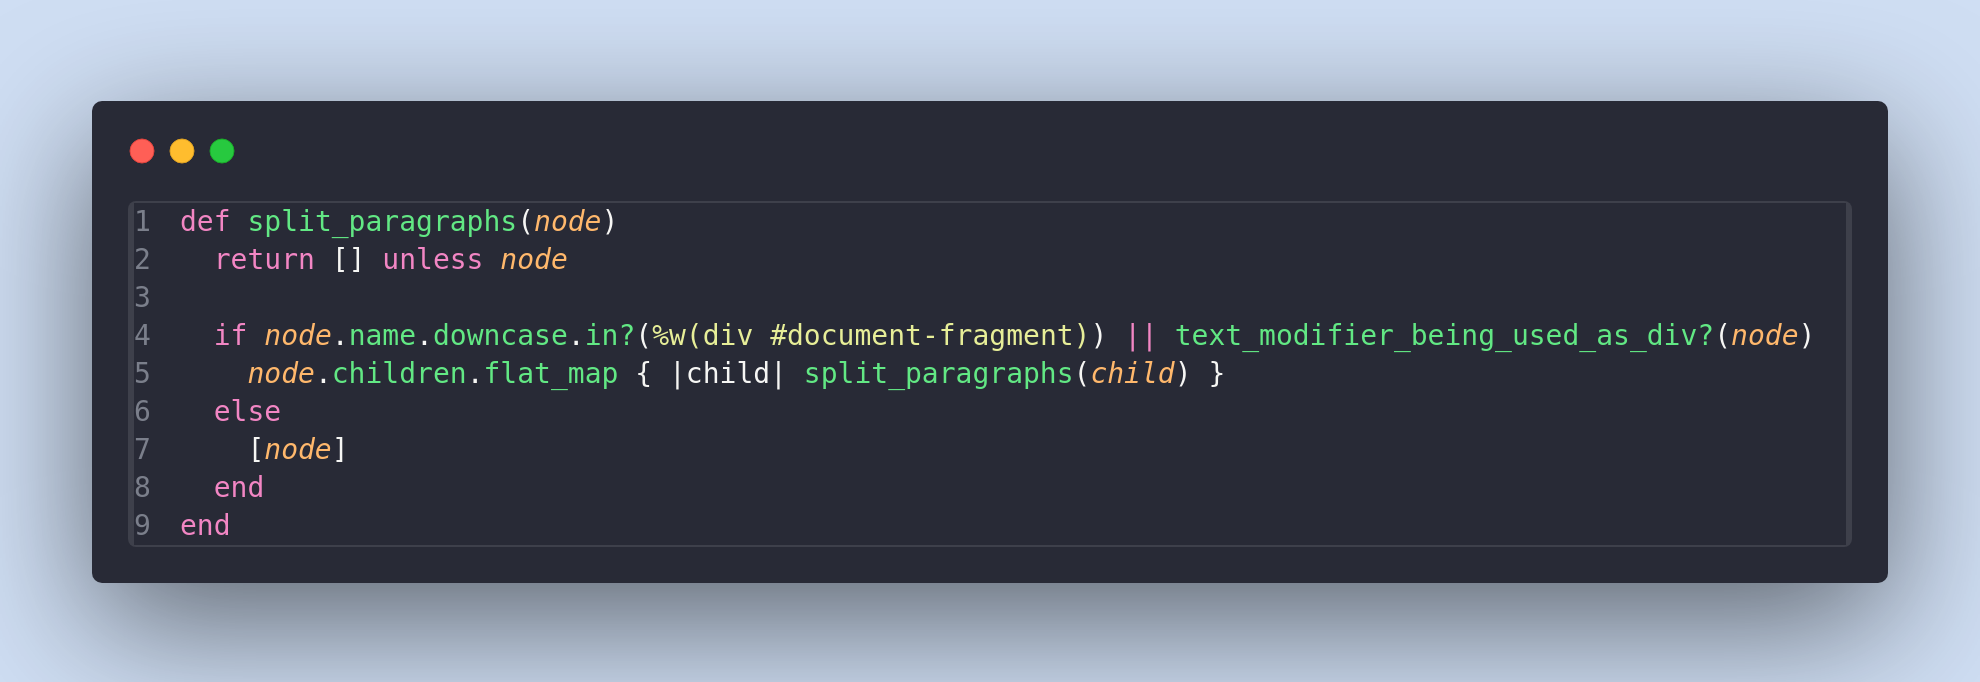
\includegraphics[width=\textwidth]{figuras/split-paragraphs-jodit.png}
  \fonte{Próprio autor}
\end{figure}

O algoritmo para definir se um determinado nó está sendo usado como \texttt{<div>} também é de caráter recursivo. A análise começa no primeiro nó passado como parâmetro. Primeiro se verifica se o nó é uma \textit{tag} modificadora de texto, se não for, o algoritmo para e a resposta é falso. Caso contrário, o algoritmo segue em frente e verifica se o nó atual possui filhos, se não tiver, ele para e a resposta é falso. Caso contrário, o algoritmo segue em frente e passa a avaliar todos os filhos diretos do nó que está sendo avaliado. Recursivamente o algoritmo irá avaliar para cada filho se este é uma \textit{tag} modificadora sendo usada como \texttt{<div>}. Se ao menos um de seus filhos for uma \textit{tag} modificadora sendo usada como \texttt{<div>}, o próprio nó também será considerado, e o algoritmo retorna verdadeiro. Na Tabela \ref{tab:tags-html-modificadoras-de-texto} está a relação de \textit{tags} que são consideradas modificadoras de texto. Vale notar que a \textit{tag} \texttt{<img>} está entre elas, pois uma imagem, nesse contexto, tem o valor semântico que um texto puro dentro de um parágrafo. Isto é, uma imagem não é fator determinante para dividir um parágrafo. O código fonte dessa verificação pode ser visto na Figura \ref{fig:text-modifier-beign-used-as-div-jodit}.

\begin{table}[h]
	\centering
	\caption{\textit{Tags} HTML modificadoras de texto}
	\label{tab:tags-html-modificadoras-de-texto}
	\begin{tabular}{c}
    \toprule
		p \\
		title \\
		span \\
		br \\
		text \\
		strong \\
		b \\
		em \\
		i \\
		u \\
		s \\
		del \\
		mark \\
		small \\
		sup \\
		code \\
		pre \\
		img \\
		a \\
		\bottomrule
	\end{tabular}
\end{table}

\begin{figure}[htbp]
  \centering
  \caption{Código fonte do método que verifica se modificador de texto está sendo usado como \texttt{<div>}}
  \label{fig:text-modifier-beign-used-as-div-jodit}
  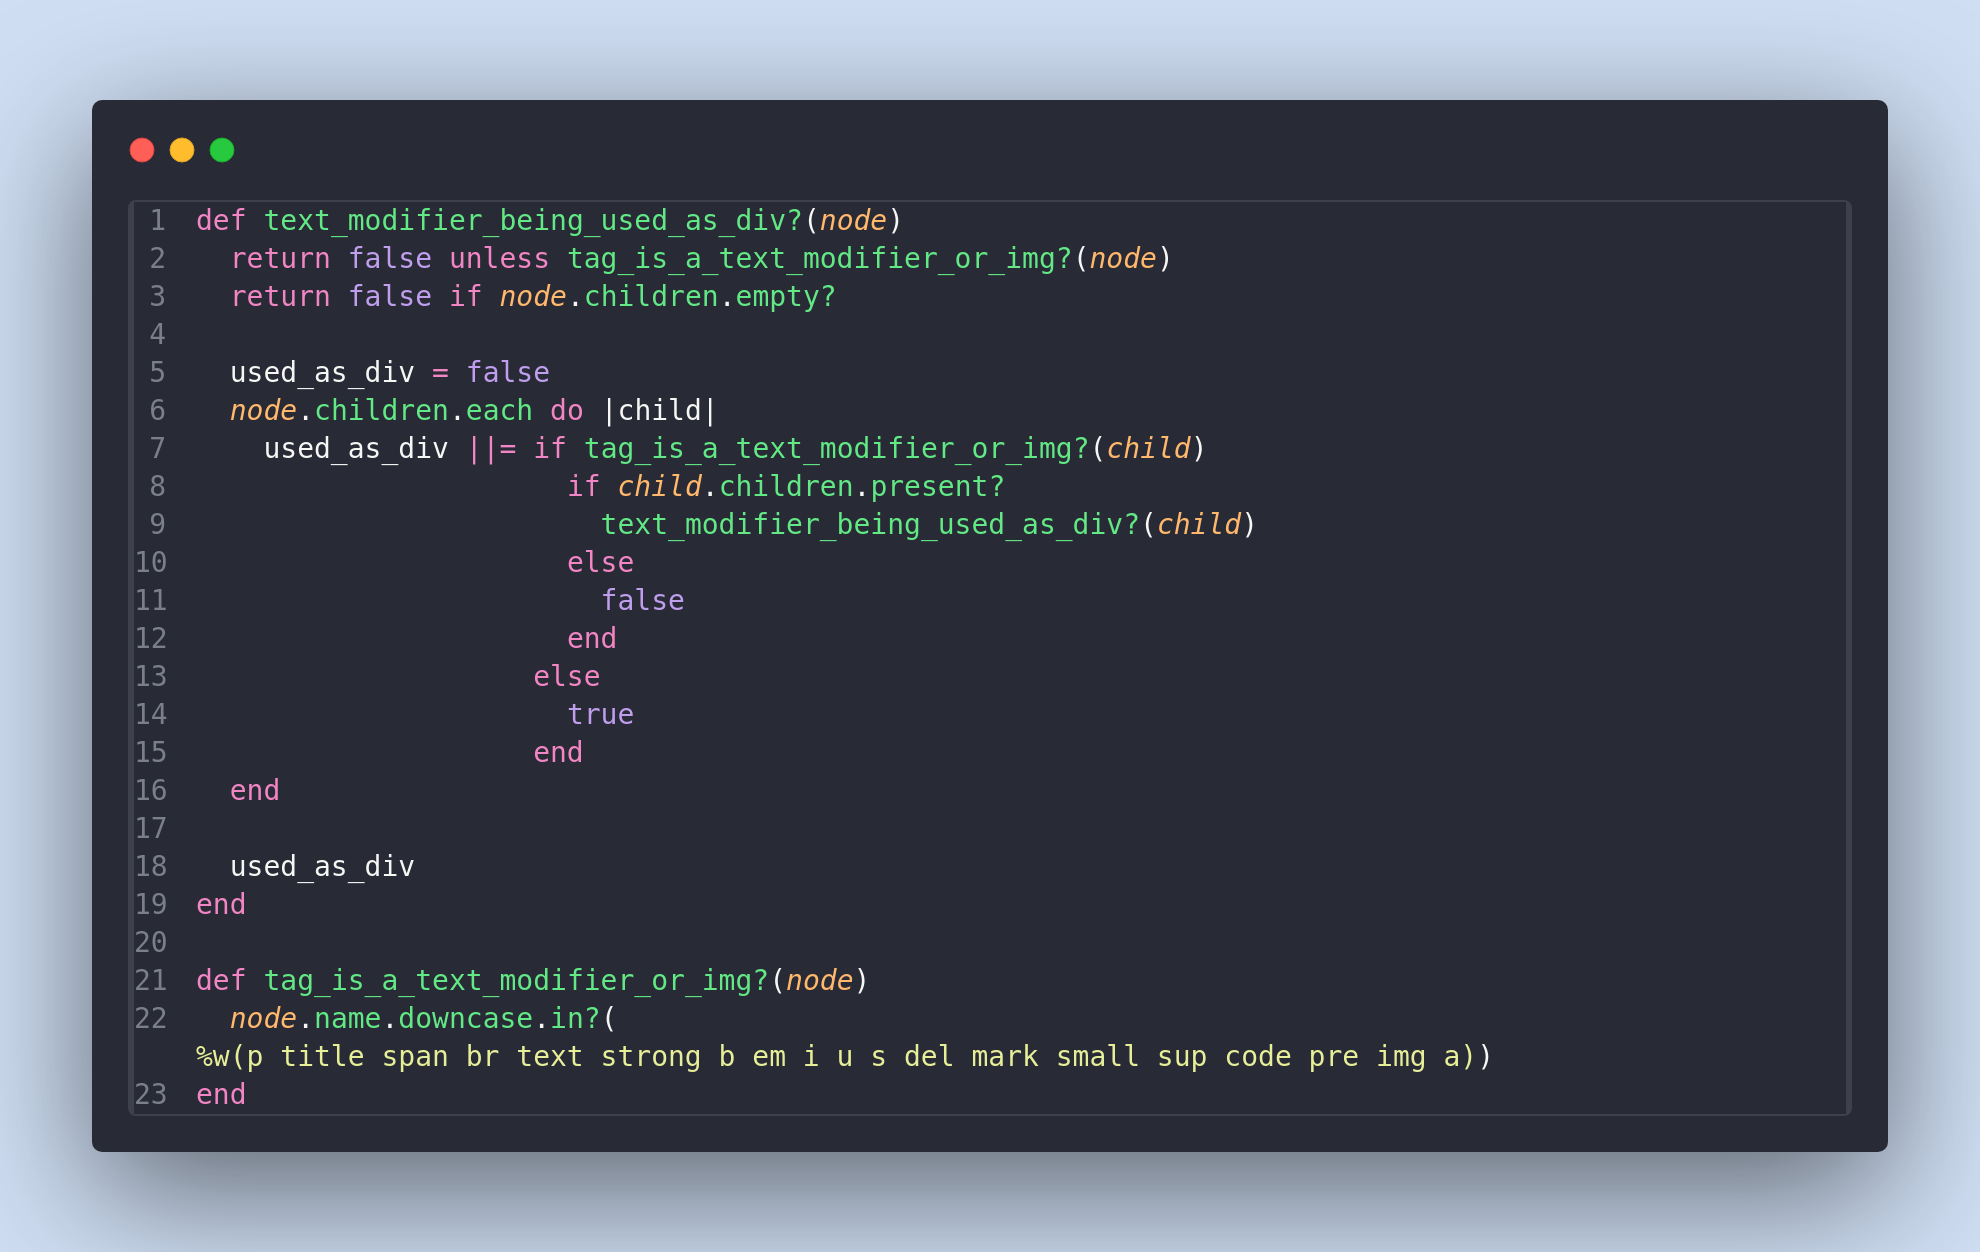
\includegraphics[width=\textwidth]{figuras/text-modifier-being-used-as-div-jodit.png}
  \fonte{Próprio autor}
\end{figure}

\section {Testes e Resultados}
\label{sec:resultados}

Os requisitos centrais das entregas realizadas neste trabalho eram sobre melhorar o desempenho das páginas de visualização e de edição do texto participativo.
Sendo assim, os testes de carga serão executados para medir quantitativamente os resultados obtidos pelas modificações realizadas na ferramenta de textos participativos do Brasil Participativo que visaram o ganho de desempenho.

É importante observar que as funcionalidades de \textit{parsing} de texto do usuário através do comando copiar e colar são completamente novas na plataforma, o que impossibilita um comparativo.

Para a execução dos testes, será utilizada a ferramenta de linha de comando \textit{Apache HTTP Server Benchmarking Tool} (ApacheBench).
Os testes serão executados em um computador com sistema operacional Linux, distribuição Ubuntu 24.04.2 LTS. As configurações de \textit{hardware} podem ser vistas na Tabela \ref{tab:especificacao-hardware-de-teste}.
Os testes utilizarão a aplicação do Brasil Participativo com execução em modo produção.
O protocolo utilizado será HTTP, e o próprio \textit{Rails} servirá os \textit{assets}.
O \textit{web-server Puma} será executado em \textit{single mode} com cinco \textit{threads}.

\begin{table}[h]
	\centering
	\caption{Especificação do hardware de teste}
	\label{tab:especificacao-hardware-de-teste}
	\begin{tabular}{cc}
    \toprule
    \textbf{Processador} & AMD Ryzen 5 7430U (6 Cores/ 12 Threads) \\
    \textbf{Placa de Vídeo} & Radeon Graphics 2GB (Integrado) \\
    \textbf{Memória RAM} & 24 GB DDR4 \\
		\bottomrule
	\end{tabular}
\end{table}

Os testes consistirão em submeter sob carga as páginas de visualização e edição do texto participativo.

Serão levantados dados para comparação com a realidade do cotidiano e os resultados dos testes apresentados pelo ApacheBench, trazendo a noção do impacto causado pelas modificações realizadas. Para trazer variabilidade nos testes, serão executados tanto os testes com volumetria de parágrafos histórica, quanto com volumetria de parágrafos extremas.

Para ambos os cenários de teste, cada parágrafo terá seu conteúdo preenchido com um texto de exemplo "\textit{Lorem Ipsum}" de 563 caracteres cada. O conteúdo utilizado será:

\textit{Lorem ipsum dolor sit amet, consectetur adipiscing elit. Sed in odio non mi auctor commodo. Aenean consequat metus massa, eget vulputate nibh suscipit vitae. Aliquam sagittis vel odio eleifend posuere. Curabitur hendrerit est elit, ac hendrerit nulla laoreet sit amet. Proin dictum tempor vulputate. Etiam cursus, quam sed cursus laoreet, dui nisi efficitur quam, at maximus dui nibh et velit. Curabitur ullamcorper ligula vitae mauris cursus rhoncus. Suspendisse laoreet felis euismod lorem accumsan, sit amet imperdiet mauris laoreet. Fusce vel tristique felis.}

A ideia central é checar o quão bem estas páginas da plataforma possivelmente operarão no dia-dia e em cenários de alta demanda.
Para os cenários extremos, será adotada a volumetria de 2 mil parágrafos por texto participativo, e 10 administradores utilizando a ferramenta paralelamente.

A versão anterior às modificações descritas neste trabalho utilizada para comparação nos testes é a \textit{tag} 1.5.0, que está disponível no respositório oficial do Brasil Participativo.

\subsection {Teste de Carga de Visualização do Rascunho}

\subsubsection {Contexto}

A fim de obter um parâmetro para comparação com teste de carga da página de edição de rascunho, foi executada no ambiente produtivo do Brasil Participativo uma consulta SQL para descobrir o dia que houveram mais criações de componentes de texto participativo. A consulta considera o período entre o primeiro dia do ano de 2024 até o último dia do mês de maio de 2025, admitindo apenas componentes que foram publicados e que são textos participativos. A consulta SQL pode ser conferida na Figura \ref{fig:consulta-top-5-dia-textos-criados}, e o seu resultado é demonstrado na Tabela \ref{tab:resultado-consulta-top-5-dia-textos-criados}.

\begin{figure}[htbp]
  \centering
  \caption{Consulta SQL para classificação dos dias com maior carga de criação de textos participativos}
  \label{fig:consulta-top-5-dia-textos-criados}
  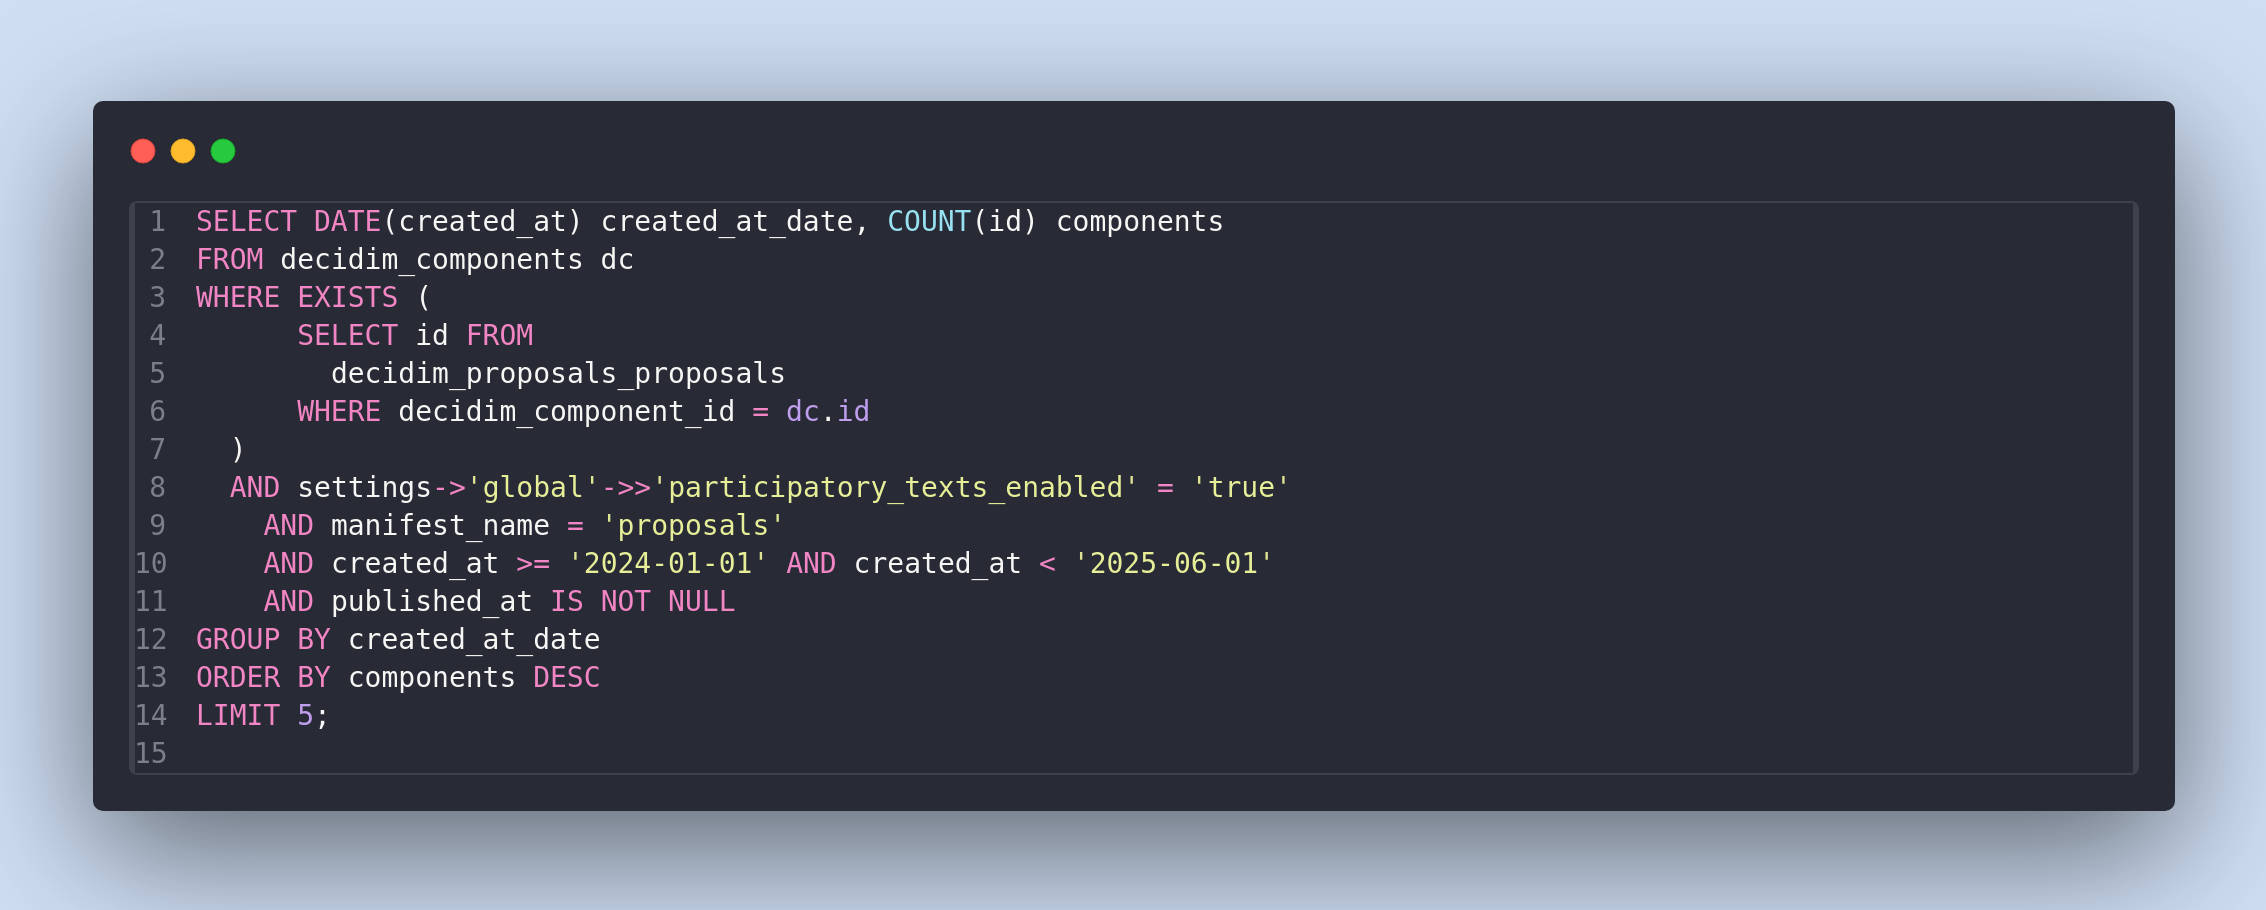
\includegraphics[width=\textwidth]{figuras/consulta-top-5-dia-textos-criados.jpg}
  \fonte{Próprio autor}
\end{figure}

\begin{table}[h]
	\centering
	\caption{Top 5 dias com maior volume de textos participativos criados}
	\label{tab:resultado-consulta-top-5-dia-textos-criados}
	\begin{tabular}{cc}
		\toprule
		\textbf{Data} & \textbf{Textos participativos criados} \\
		\midrule
    29/11/2024 & 45 \\
    30/11/2024 & 24 \\
    02/12/2024 & 17 \\
    22/01/2025 & 15 \\
    09/10/2024 & 12 \\
		\bottomrule
	\end{tabular}
  \fonte{Próprio autor}
\end{table}

No dia 29 de novembro de 2024, houveram 45 componentes de texto participativo criados na plataforma. Uma segunda consulta foi executada para descobrir a classificação dos cinco textos participativos dessa data com a maior quantidade de parágrafos. A consulta SQL pode ser conferida na Figura \ref{fig:consulta-top-textos-participativos-paragrafos}, e o seu resultado na Tabela \ref{tab:resultado-consulta-top-textos-participativos-paragrafos}. Nota-se que para essa data, o texto participativo com a maior quantidade de parágrafos foi de 124.

\begin{figure}[htbp]
  \centering
  \caption{Consulta SQL para classificação dos textos participativos com maior quantidade de parágrafos}
  \label{fig:consulta-top-textos-participativos-paragrafos}
  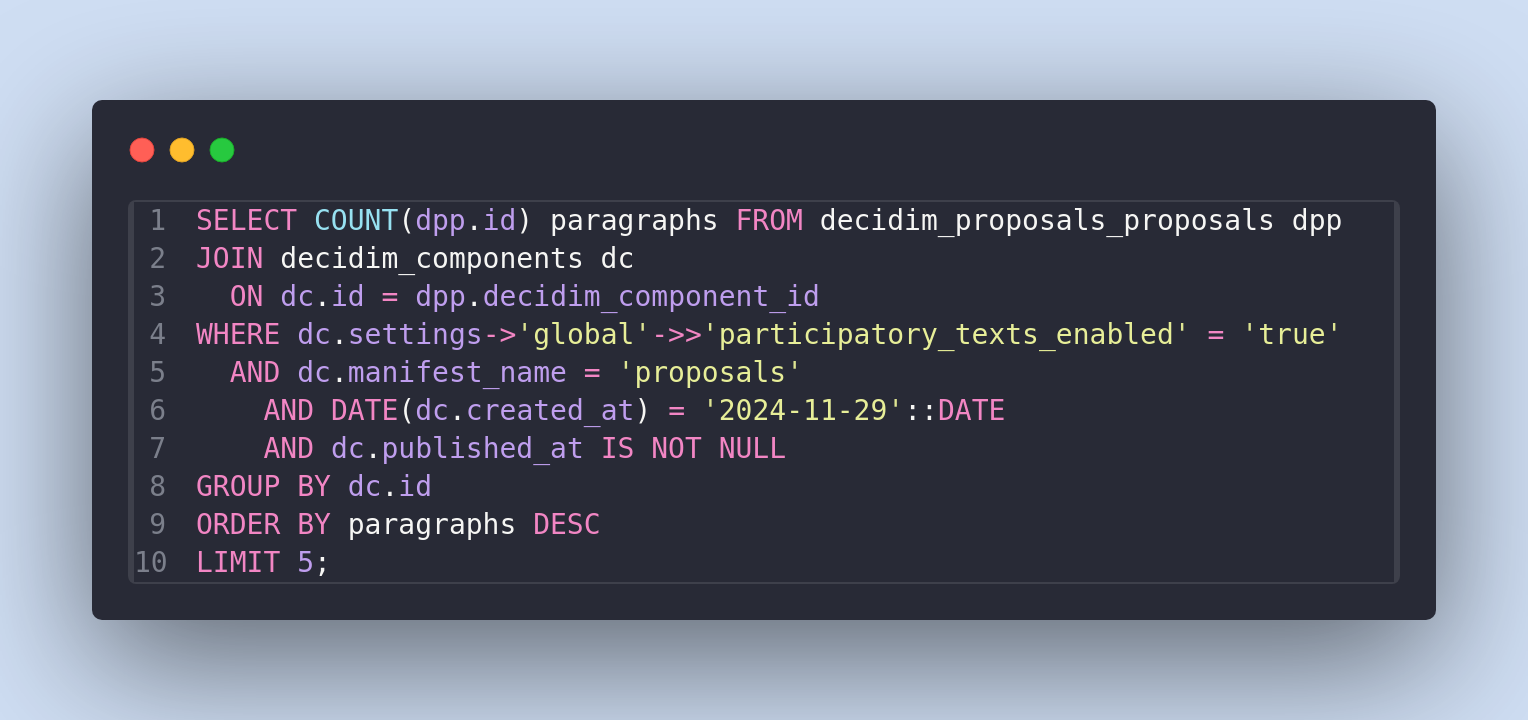
\includegraphics[width=\textwidth]{figuras/consulta-top-textos-participativos-paragrafos.png}
  \fonte{Próprio autor}
\end{figure}

\begin{table}[h]
	\centering
	\caption{Top 5 textos participativos de 29/11/2024 com maior volume de parágrafos}
	\label{tab:resultado-consulta-top-textos-participativos-paragrafos}
	\begin{tabular}{c}
		\toprule
		\textbf{Parágrafos} \\
		\midrule
    124 \\
    85  \\
    80 \\
    76 \\
    74 \\
		\bottomrule
	\end{tabular}
  \fonte{Próprio autor}
\end{table}

Com base nessas informações, será considerado um dia com pico de uso com 50 componentes sendo criados, cada um deles com 130 parágrafos.
Será levado em conta que o usuaŕio administrador possivelmente trabalha na plataforma entre os horários das nove horas da manhã até meio dia (12 horas), e das 13 horas até às 18 horas, significando uma janela de trabalho de oito horas. O que significa em aproximadamente de seis a sete componentes criados por hora.

Assumindo um possível pior cenário, também por convenção, será considerado que o administrador realiza em média no mínimo todas as cinco operações em cada parágrafo, isto é: editar, mesclar, mover, ocultar e desabilitar interações.
Para este teste será ignorado o fato de que a operação de mesclagem diminui a contagem de parágrafos em uma unidade.
A realização de cada operação acarreta na atualização da página de visualização do rascunho, portanto considerando os seis a sete componentes por hora (nesse caso será considerado sete, simplesmente), a quantidade de 150 parágrafos e as cinco operações por parágrafo, tem-se que a página de visualização do rascunho será renderizada 5.250 vezes em uma hora, ou 87 vezes por minuto, ou 1,46 vezes por segundo.

\subsubsection {Execução e Resultados}

Os testes foram realizados disparando 100 requisições com o fator de paralelismo igual a cinco, isto é, ocupando todas as cinco threads do servidor cada uma com um único usuário. Os resultados podem ser visualizados na Tabela \ref{tab:teste-carga-visualizar-rascunho}

\begin{table}[h]
	\centering
	\caption{Teste da página de edição do texto}
	\label{tab:teste-carga-visualizar-rascunho}
	\begin{tabular}{ccc}
		\toprule
		Métrica & Versão anterior & \textbf{Nova versão} \\
		\midrule
    \textbf{Tamanho da página} & 931.752 bytes & 712.295 bytes \\
    \textbf{Tempo gasto no teste} & 109 segundos & 18 segundos \\
    \textbf{Requisições por segundo} & 0,91 & 5,38 \\
    \textbf{Tempo médio por requisição} & 1.097 milissegundos & 185 milissegundos \\
		\bottomrule
	\end{tabular}
  \fonte{Próprio autor}
\end{table}

\subsubsection {Testes Extremos}

Os testes extremos foram realizados com 10 requisições com fator de paralelismo igual a 10. O número de requisições foi escolhido como 10 para garantir que os testes ocorressem em uma escala de tempo na casa de alguns minutos, evitando problemas de expiração de sessão, dado que o teste foi realizado usando um Cookie de sessão de usuário administrador extraído do navegador manualmente. O texto participativo utilizado possui 2 mil parágrafos. Os resultados podem ser conferidos na Tabela \ref{tab:teste-carga-extremo-visualizar-rascunho}.

\begin{table}[h]
	\centering
	\caption{Teste extremo da página de edição do texto}
	\label{tab:teste-carga-extremo-visualizar-rascunho}
	\begin{tabular}{ccc}
		\toprule
		Métrica & Versão anterior & \textbf{Nova versão} \\
		\midrule
    \textbf{Tamanho da página} & 14.027.611 bytes & 5.888.914 bytes \\
    \textbf{Tempo gasto no teste} & 158 segundos & 20 segundos \\
    \textbf{Requisições por segundo} & 0,06 & 0,48 \\
    \textbf{Tempo médio por requisição} & 15.837 milissegundos & 2.084 milissegundos \\
		\bottomrule
	\end{tabular}
  \fonte{Próprio autor}
\end{table}

\subsection {Teste de Carga de Visualização do Texto}

\subsubsection {Execução e Resultados}

Os testes foram realizados disparando 100 requisições com o fator de paralelismo igual a cinco. Os resultados podem ser visualizados na Tabela \ref{tab:teste-carga-visualizar-texto}. Para esse teste não se faz necessário o uso de Cookie de sessão de usuário, uma vez que a página é pública e possível de visualizar sem estar logado na plataforma.

\begin{table}[h]
	\centering
	\caption{Teste da página de visualização do texto}
	\label{tab:teste-carga-visualizar-texto}
	\begin{tabular}{ccc}
		\toprule
		Métrica & Versão anterior & \textbf{Nova versão} \\
		\midrule
    \textbf{Tamanho da página} & 437.372 & 528.236 \\
    \textbf{Tempo gasto no teste} & 455 segundos & 15 segundos \\
    \textbf{Requisições por segundo} & 0,22 & 6,61 \\
    \textbf{Tempo médio por requisição} & 4.551 milissegundos & 151 milissegundos \\
		\bottomrule
	\end{tabular}
  \fonte{Próprio autor}
\end{table}

\subsubsection {Testes Extremos}

\begin{table}[h]
	\centering
	\caption{Teste extremo da página de visualização do texto}
	\label{tab:teste-carga-extremo-visualizar-texto}
	\begin{tabular}{ccc}
		\toprule
		Métrica & Versão anterior & \textbf{Nova versão} \\
		\midrule
    \textbf{Tamanho da página} & 2.510.864 bytes & 3.239.958 bytes \\
    \textbf{Tempo gasto no teste} & 503 segundos & 16 segundos \\
    \textbf{Requisições por segundo} & 0,02 & 0,61 \\
    \textbf{Tempo médio por requisição} & 50.345 milissegundos & 1.644 milissegundos \\
		\bottomrule
	\end{tabular}
  \fonte{Próprio autor}
\end{table}

\subsection {Resultados Gerais}

As alterações abordadas neste trabalho foram devidamente incluídas no código fonte do Brasil Participativo e utilizadas no ambiente produtivo. Até o presente momento a ferramenta está sendo utilizada e posta à prova. Considera-se como um sucesso o atingimento de todos os requisitos levantados dado fato que foi realizada uma cerimonia de validação juntamente com o time de produto do Lab Livre.

\chapter {Considerações Finais}

Este trabalho teve como objetivo demonstrar a explorar uma jornada de desenvolvimento de funcionalidades levando em consideração requisitos levantados por \textit{stakeholders} e outros times, tendo como foco principal o desenvolvimento de funcionalidades com requisitos de desempenho mais rigorosos.

A metodologia adotada se baseou no desenvolvimento continuo, onde em cada ciclo de desenvolvimento novos requisitos eram priorizados e executados. A mudança de escopo, apesar de não ser o foco de detalhamento desse trabalho, foi algo presente na jornada de desenvolvimento, mas em nenhum momento foi impeditivo para realização de entregas.

Apesar do enfoque em otimização de desempenho, muitos outros tópicos relacionados ao desenvolvimento foram abordados, trazendo maior profundidade em relação às contribuições realizadas no projeto.

É esperado que a medida que a funcionalidade seja utilizada por usuários reais, correções e ajustes sejam feitos pelo time desenvolvimento do Lab Livre, trazendo maior maturidade e grau de confiança na solução.

Muitos dos tópicos aqui abordados podem vir a ser objeto de evolução futuramente, principalmente em relação a desempenho.

Sabe-se que ainda há oportunidades de desenvolvimento que potencialmente trarão melhorias de desempenho para a plataforma e para a ferramenta de textos participativos.
Como mencionado, existem diversos outros problemas de desempenho em partes específicas do sistema.

